\chapter{Simulation Results}
\label{sec:simulation_results}

All the designs presented in \Cref{sec:comparison} are tested in simulation.
As explained in \Cref{sec:method}, they are simulated in
Gazebo$^\textrm{\textregistered}$ and controlled by the means of a ROS node.
These simulations are performed to evaluate the feasibility and  the controllability
of the theoretical optimal designs obtained in \Cref{sec:optimization_results}.
As a first result it is important to state that all the MAVs tested in simulation
were controlled properly and could maneuver well. Hence, all the optimal designs
presented in \Cref{sec:comparison} from the tri-copter to the octa-copter are
feasible.
The simulations also allow for comparison between different MAVs' dynamical abilities.\\
In this section the most interesting simulation results obtained are presented.
First, a flight test performed by the tri-copter depicted in \Cref{fig:comp_tri} is
presented, then a comparison between the hexa-copter shown in \Cref{fig:comp_hexa}
and the Voliro from \citep{kamel_voliro:_2018} is proposed. Finally, a manipulation
example with the hepta-copter presented in \Cref{sec:hepta_copter} is shown.

\section{Tri-copter}
\label{sec:tri_copter_sim}

The tri-copter with tilting rotor is a very interesting case because it is holonomic,
which means that it has exactly six degrees of freedom (DoF) and evolves in a
three dimensional space. Therefore, it should theoretically be able to produce forces
and torques in any direction. To verify that a test flight is performed where the MAV
hovers at one meter above the ground and changes its orientation up to a pitch angle
$\theta$ equal to $90^{\circ}$. The results of this test can be observed in
\Cref{fig:tri_sim} and this observation of a quarter pitch flip illustrates the fact
that the tri-copter is indeed able to hover in any orientation.

\begin{figure}[!ht]
  \begin{center}
  \begin{minipage}[t]{0.24\textwidth}
    \centering
    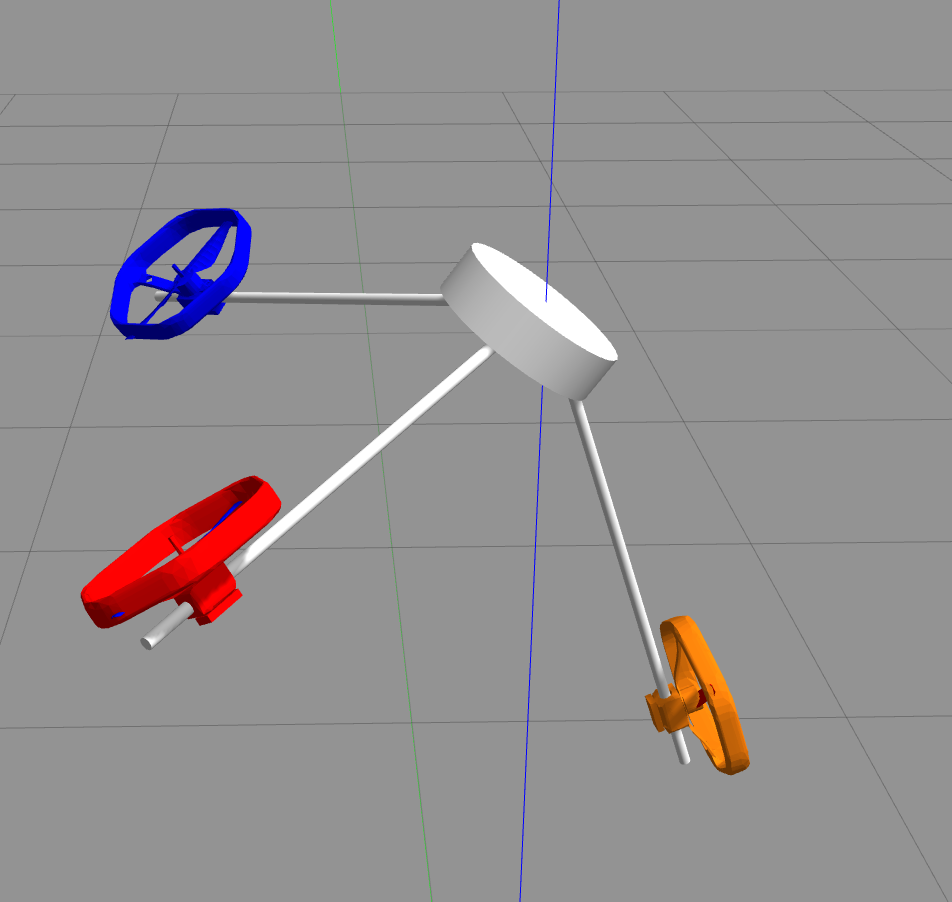
\includegraphics[width=\linewidth]{images/tri_sim1.png}
  \end{minipage}
  \hfill
  \begin{minipage}[t]{0.24\textwidth}
    \centering
    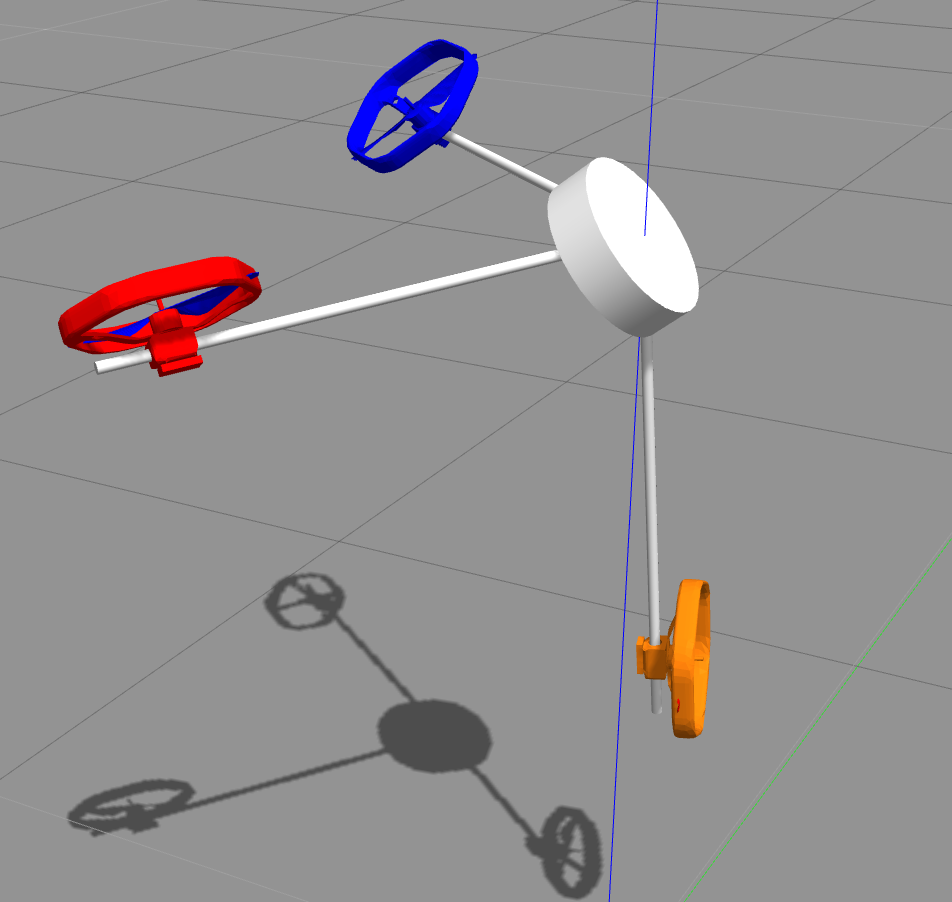
\includegraphics[width=\linewidth]{images/tri_sim2.png}
  \end{minipage}
  \hfill
  \begin{minipage}[t]{0.24\textwidth}
    \centering
    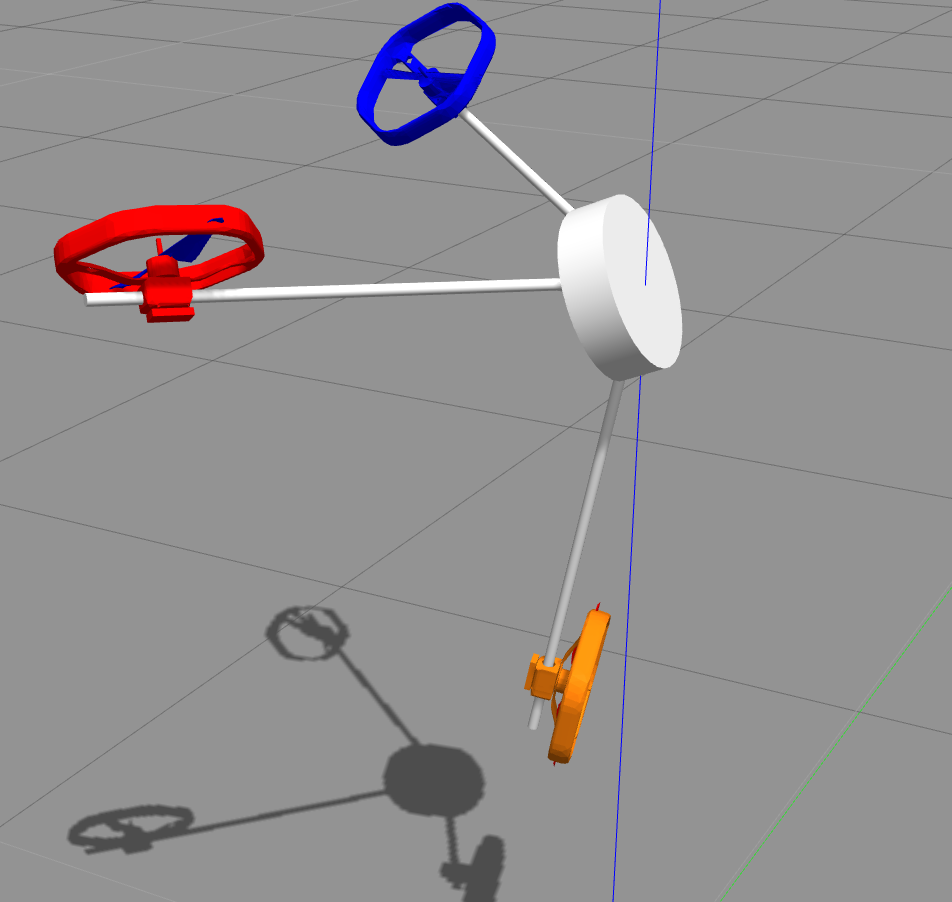
\includegraphics[width=\linewidth]{images/tri_sim3.png}
  \end{minipage}
  \hfill
  \begin{minipage}[t]{0.24\textwidth}
    \centering
    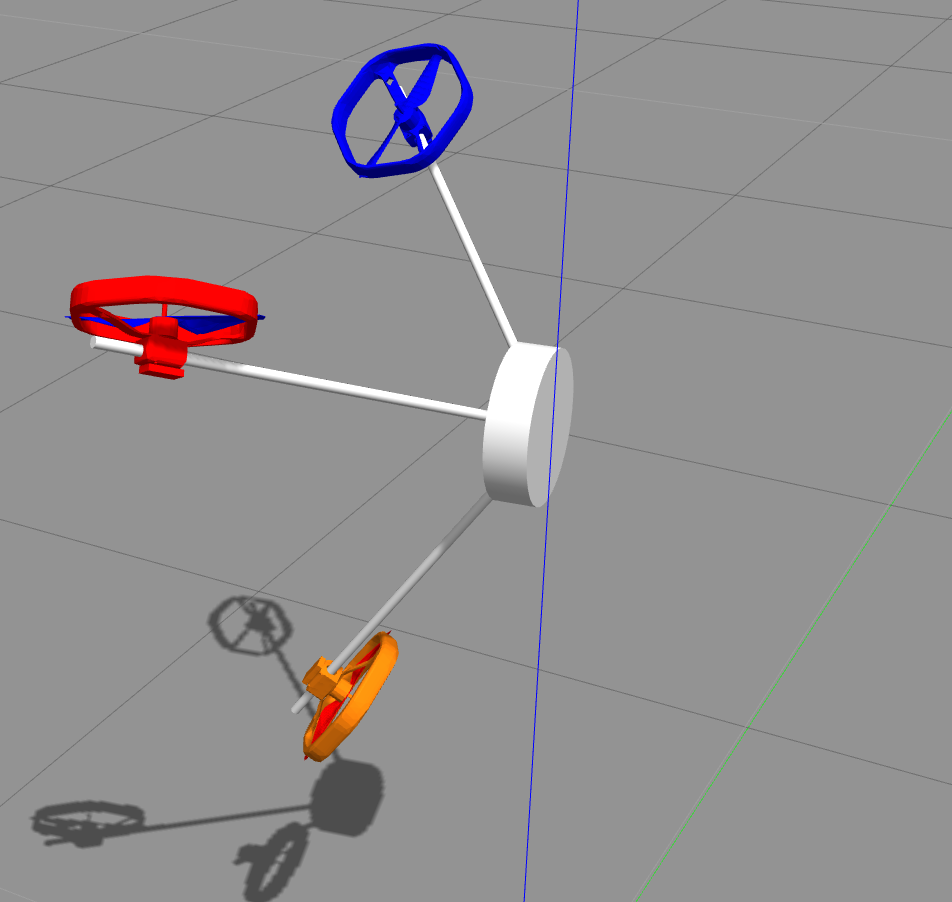
\includegraphics[width=\linewidth]{images/tri_sim4.png}
  \end{minipage}
  \caption{Simulation of the tri-copter in Gazebo.}
  \label{fig:tri_sim}
  \end{center}
\end{figure}

\clearpage

\section{Hexa-copter}
\label{sec:hexa_copter_sim}

The aim of this section is to compare the abilities of Voliro shown in
\Cref{fig:Voliro_sim} with those of the optimal hexa-copter shown in \Cref{fig:Hexa_sim}.
In order to do so, two maneuvers were performed with each of the MAVs in
Gazebo$^\textrm{\textregistered}$.

\begin{figure}[!ht]
  \resizebox{\textwidth}{!}{\begin{subfigure}[b]{0.5\textwidth}
    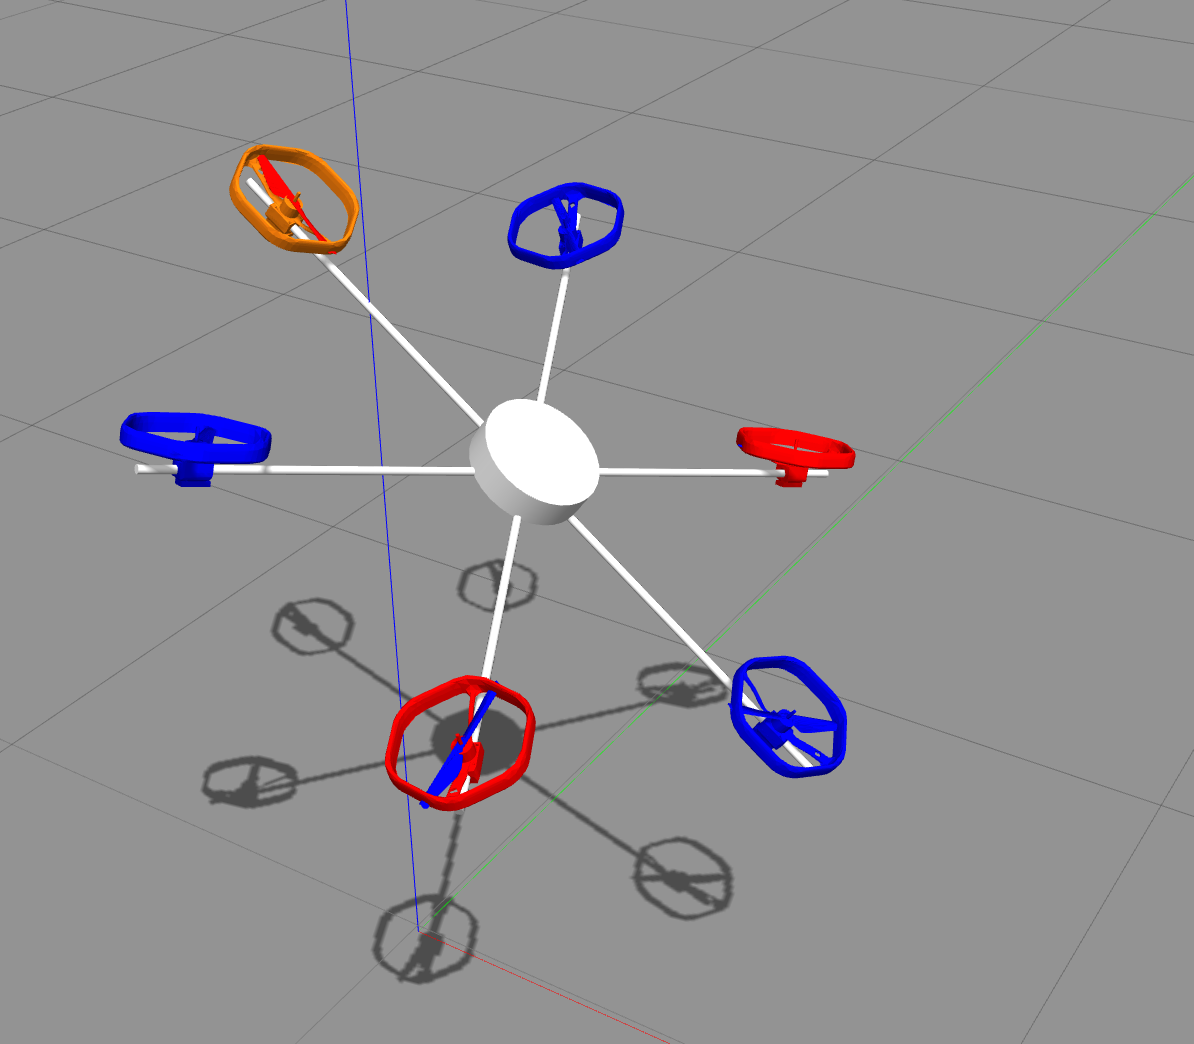
\includegraphics[width=\linewidth]{images/Voliro_sim.png}
    \caption{Voliro.} \label{fig:Voliro_sim}
  \end{subfigure}
  \hspace*{\fill} % separation between the subfigures
  \begin{subfigure}[b]{0.5\textwidth}
    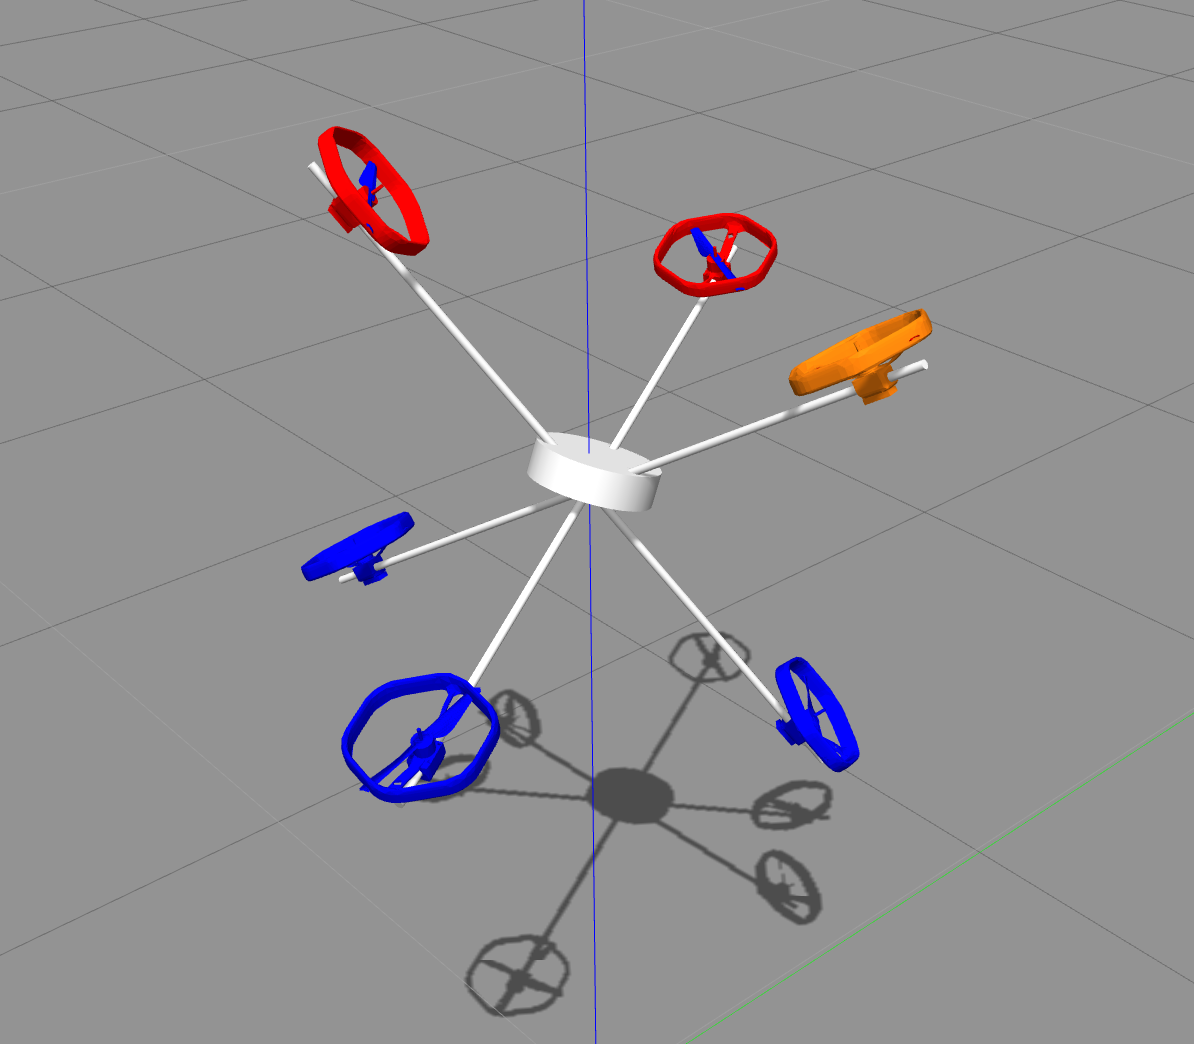
\includegraphics[width=\linewidth]{images/Hexa_sim.png}
    \caption{Optimal hexa-copter.} \label{fig:Hexa_sim}
  \end{subfigure}}
  \caption{Representation of two six-rotor MAV models spawned in Gazebo$^\textrm{\textregistered}$.}
  \label{fig:Sim_six_rotors}
\end{figure}

The first maneuver was a position tracking exercise, where the drones followed a
trajectory describing two rounds of a circle, one meter above the ground at a speed
of $0.63\ [\frac{m}{s}]$. The graphs shown in \Cref{fig:Voliro_position_circle} and
\Cref{fig:Hexa_position_circle} are the trajectory tracking plots.
The graphs in \Cref{fig:Voliro_angle_circle} and \Cref{fig:Hexa_angle_circle}
illustrate the orientation errors produced by the MAVs while following
this circular trajectory.
The second maneuver was an orientation tracking exercise, where the drones took off,
hovered one meter above the ground for a few seconds, and then performed a full
pitch flip, to finally land. The graphs shown in \Cref{fig:Voliro_position_pitch}
and \Cref{fig:Hexa_position_pitch} are the trajectory tracking plots of this maneuver.
The graphs in \Cref{fig:Voliro_angle_pitch} and \Cref{fig:Hexa_angle_pitch} illustrate
the orientation tracking plot of the pitch flip.\\
First, when comparing \Cref{fig:Voliro_position_circle} with
\Cref{fig:Hexa_position_circle} it is noteworthy that the optimal hexa-copter
tracks the position with less delay. Then, when comparing \Cref{fig:Voliro_angle_circle}
with \Cref{fig:Hexa_angle_circle}, one can notice that even though the orientation
error is very small for both designs, Voliro’s is jittering more and slightly larger.
When looking at the orientation tracking graphs in \Cref{fig:Voliro_angle_pitch}
and in \Cref{fig:Hexa_angle_pitch}, it is interesting to see that both designs
performed well in this exercise. However, in \Cref{fig:Voliro_angle_pitch}
there are two small overshoots in the orientation tracking. This is due to
the fact that the controller uses the static allocation described in \Cref{sec:allocation}
to compute the desired tilting angles and speed for the rotors. This static matrix
becomes singular in certain orientations and it leads to the loss of full-actuation in
those orientations. This happens among others when on arm is oriented vertically.
One can notice that this orientational instability happened only once for
the hexa-copter’s pitch flip (see \Cref{fig:Hexa_angle_pitch}). This is because
the hexa-copter only has one arm oriented vertically when performing the
pitch flip. It is a consequence of the even distribution of the propellers
in the space around the body that makes this MAV’s dynamical properties
really balanced.


\begin{figure}[!ht]
  \begin{center}
    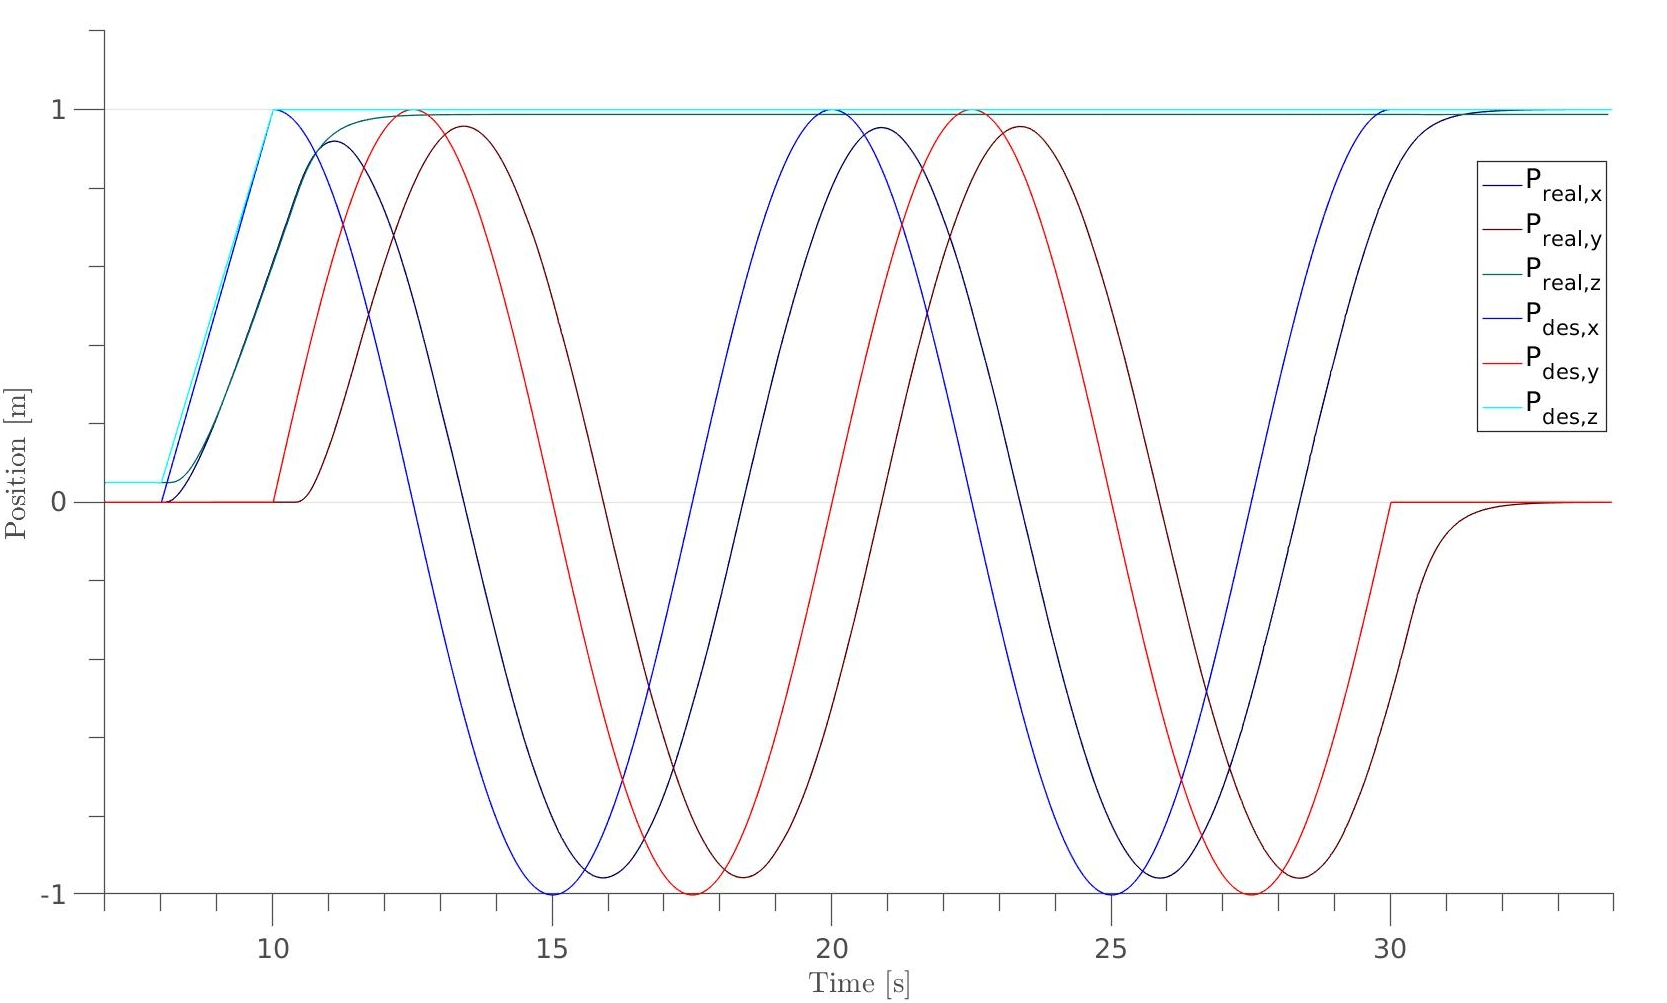
\includegraphics[width=1.0\linewidth]{images/Voliro_circle_position.jpg}
    \caption{Trajectory tracking of a one meter circle performed by Voliro.}
    \label{fig:Voliro_position_circle}
  \end{center}
\end{figure}

\begin{figure}[!ht]
  \begin{center}
    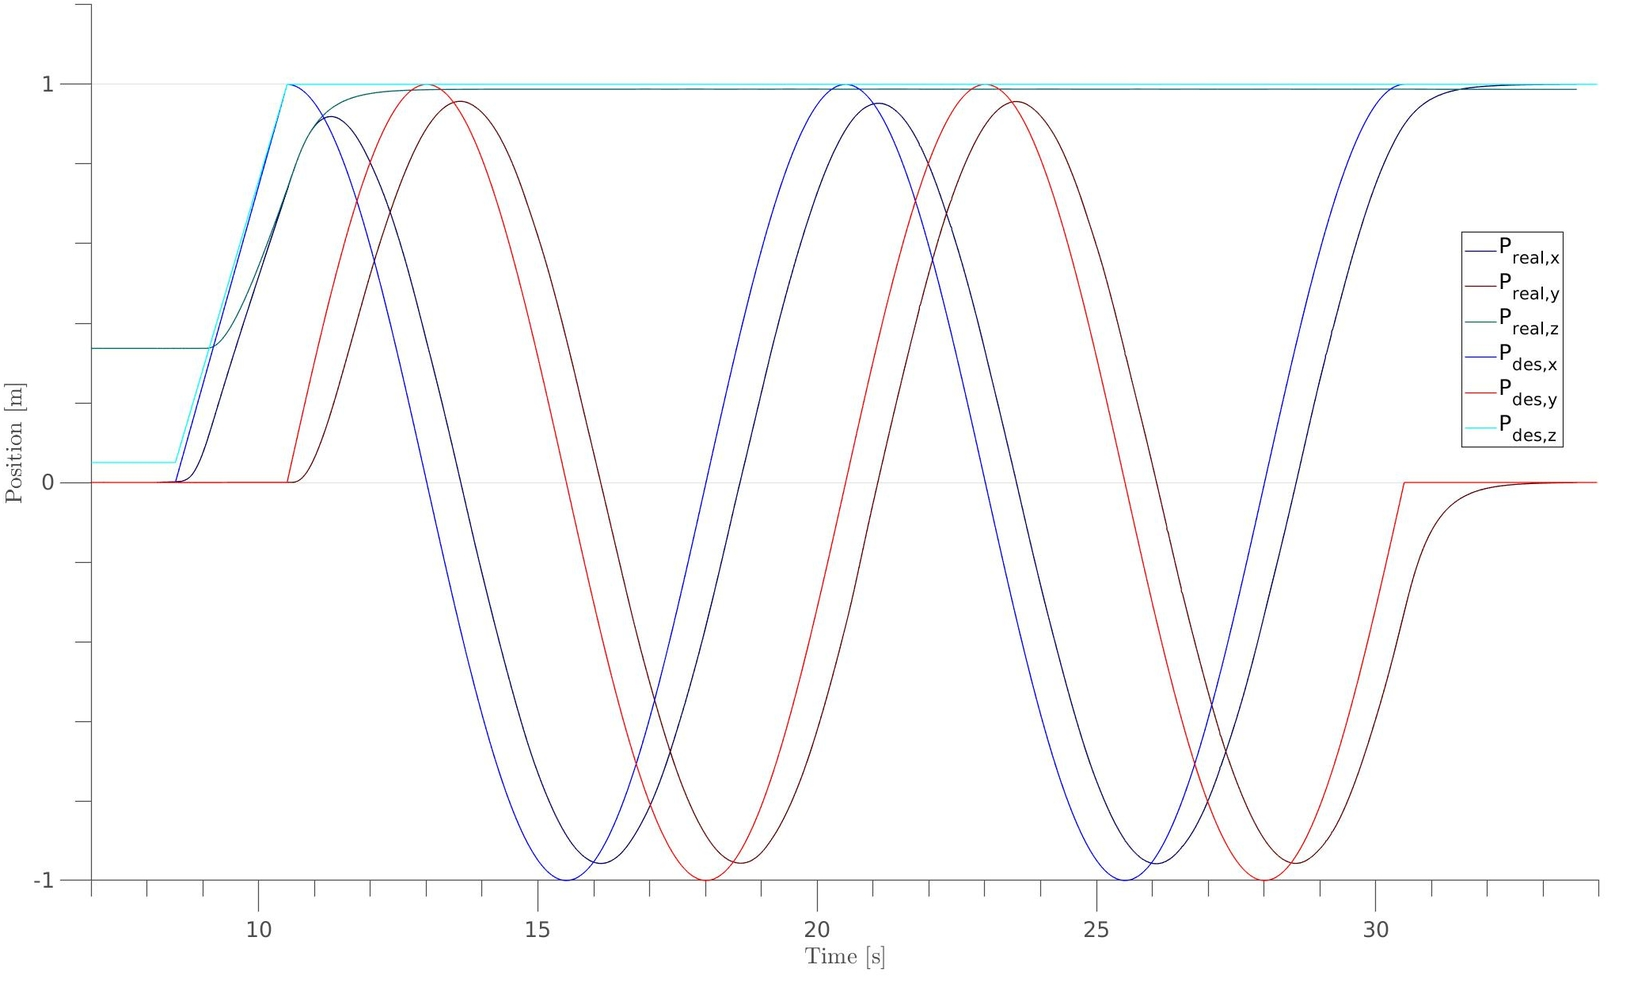
\includegraphics[width=1.0\linewidth]{images/Hexa_circle_position.jpg}
    \caption{Trajectory tracking of a one meter circle performed by the optimal hexa-copter.}
    \label{fig:Hexa_position_circle}
  \end{center}
\end{figure}

\begin{figure}[!ht]
  \begin{center}
    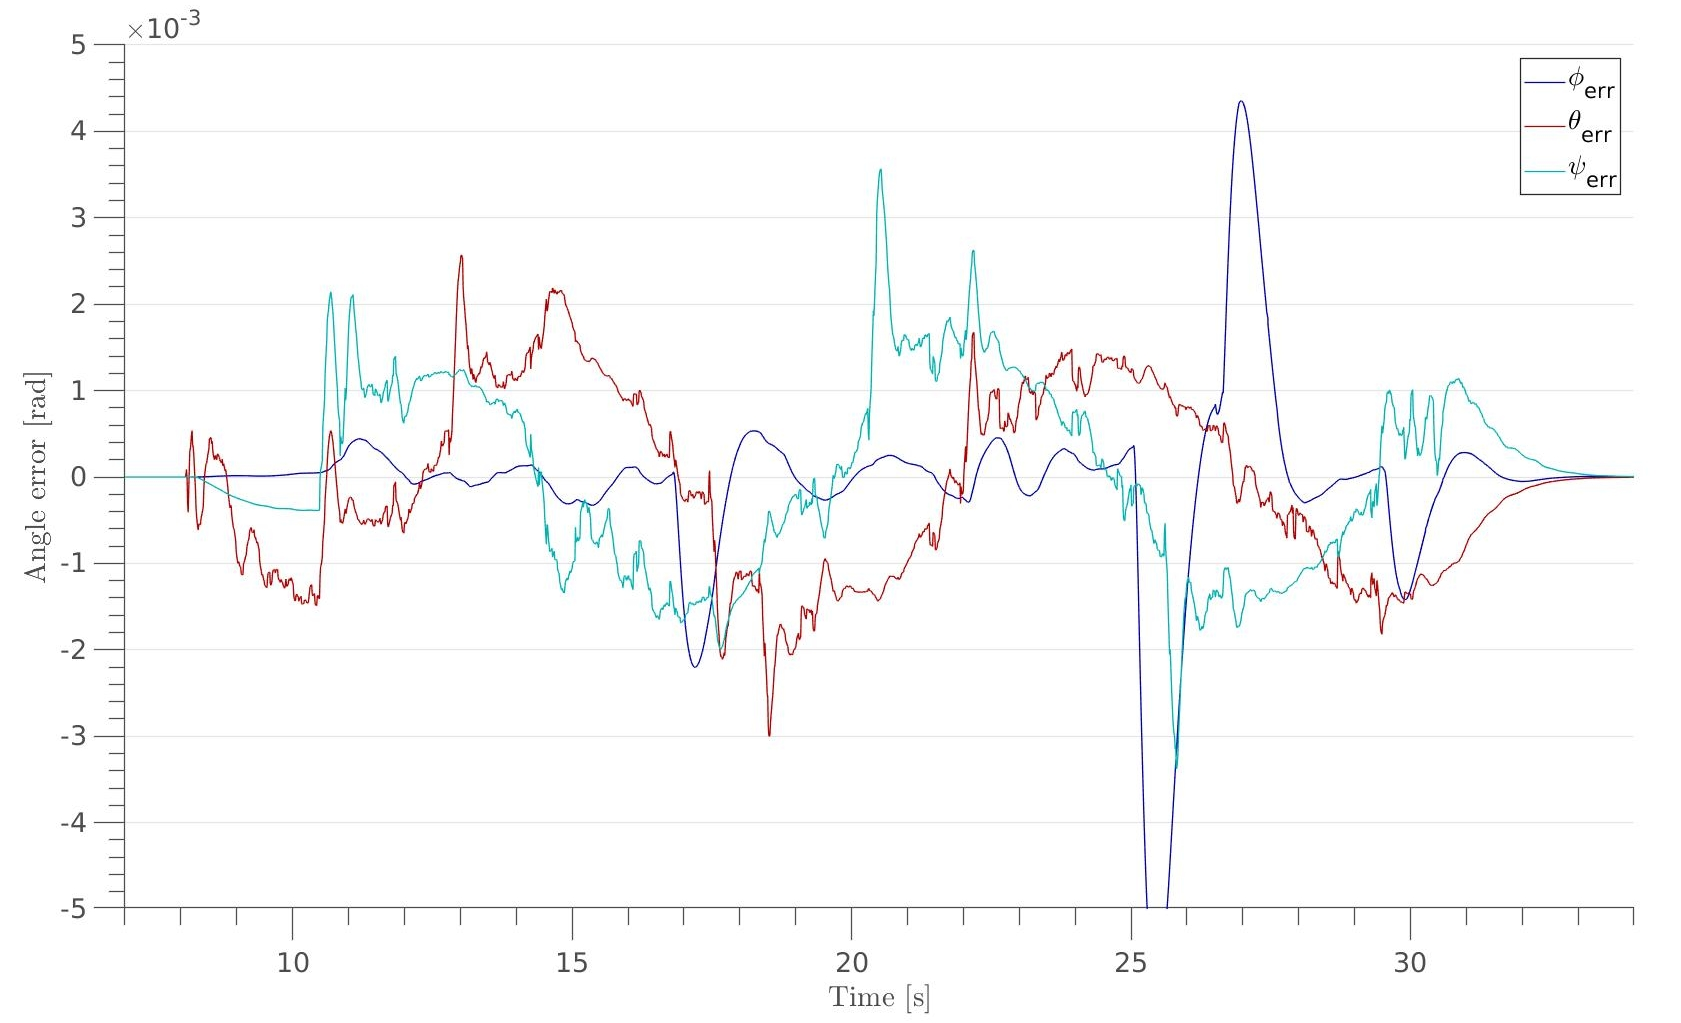
\includegraphics[width=1.0\linewidth]{images/Voliro_circle_angle.jpg}
    \caption{Pitch, roll and yaw angle errors when Voliro tracks a one meter circle.}
    \label{fig:Voliro_angle_circle}
  \end{center}
\end{figure}

\begin{figure}[!ht]
  \begin{center}
    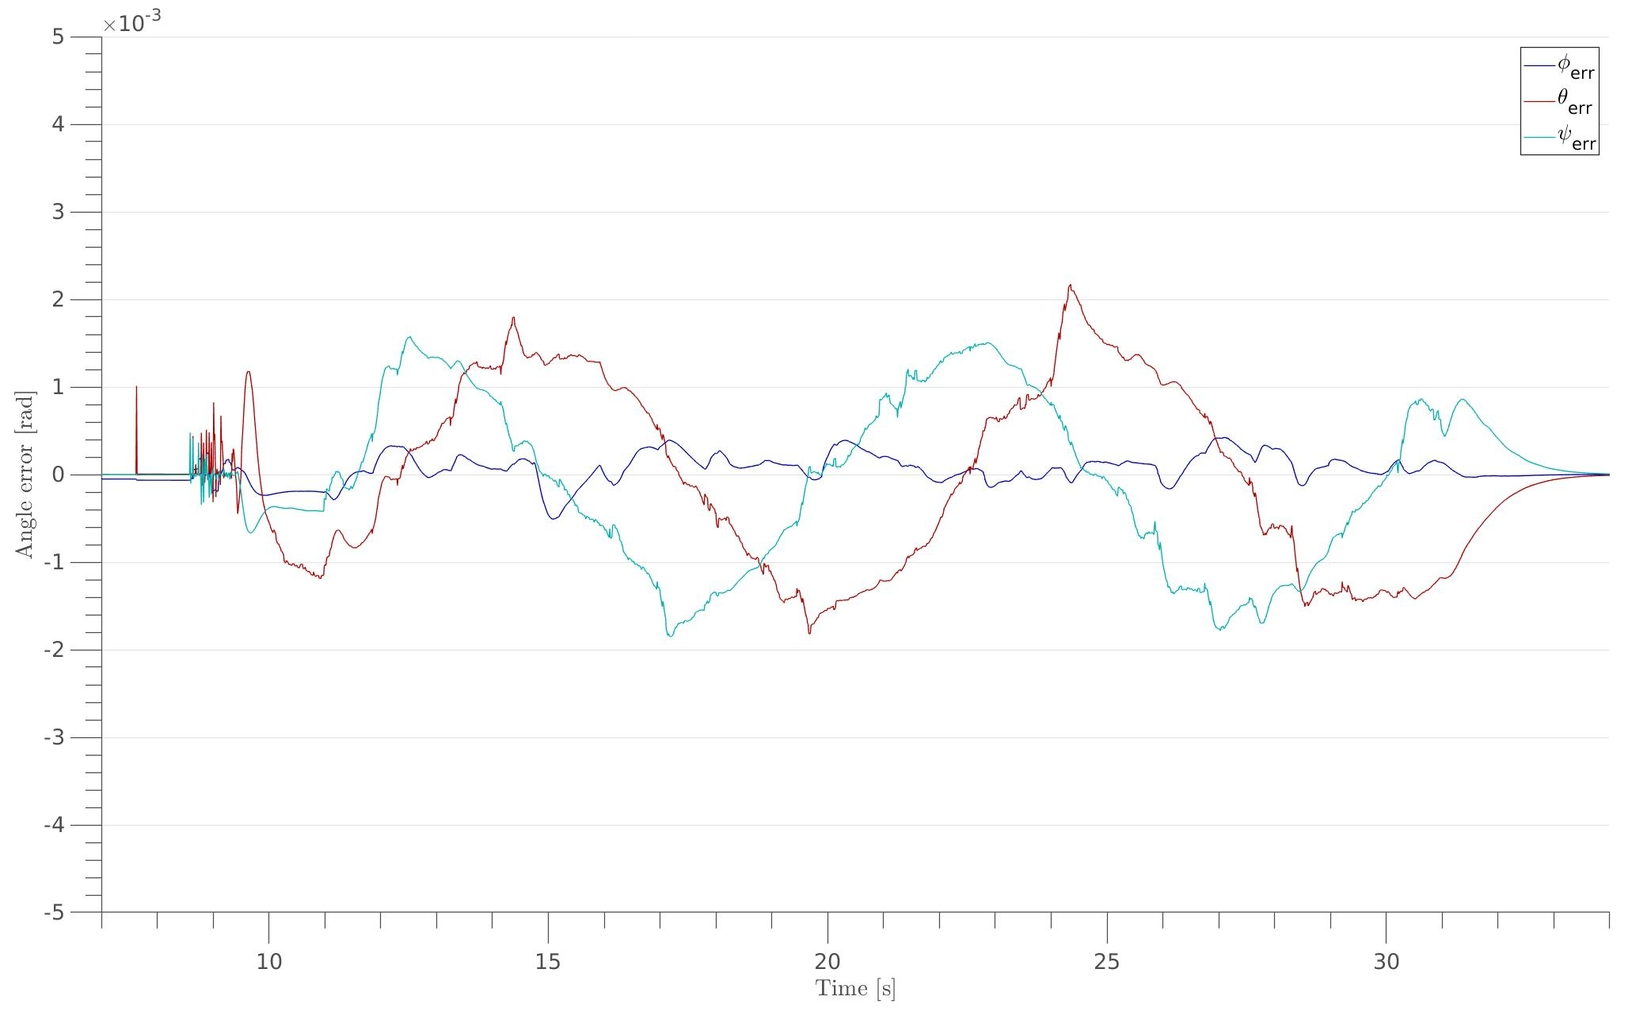
\includegraphics[width=1.0\linewidth]{images/Hexa_circle_angle.jpg}
    \caption{Pitch, roll and yaw angle errors when the optimal hexa-copter tracks a one meter circle.}
    \label{fig:Hexa_angle_circle}
  \end{center}
\end{figure}

\begin{figure}[!ht]
  \begin{center}
    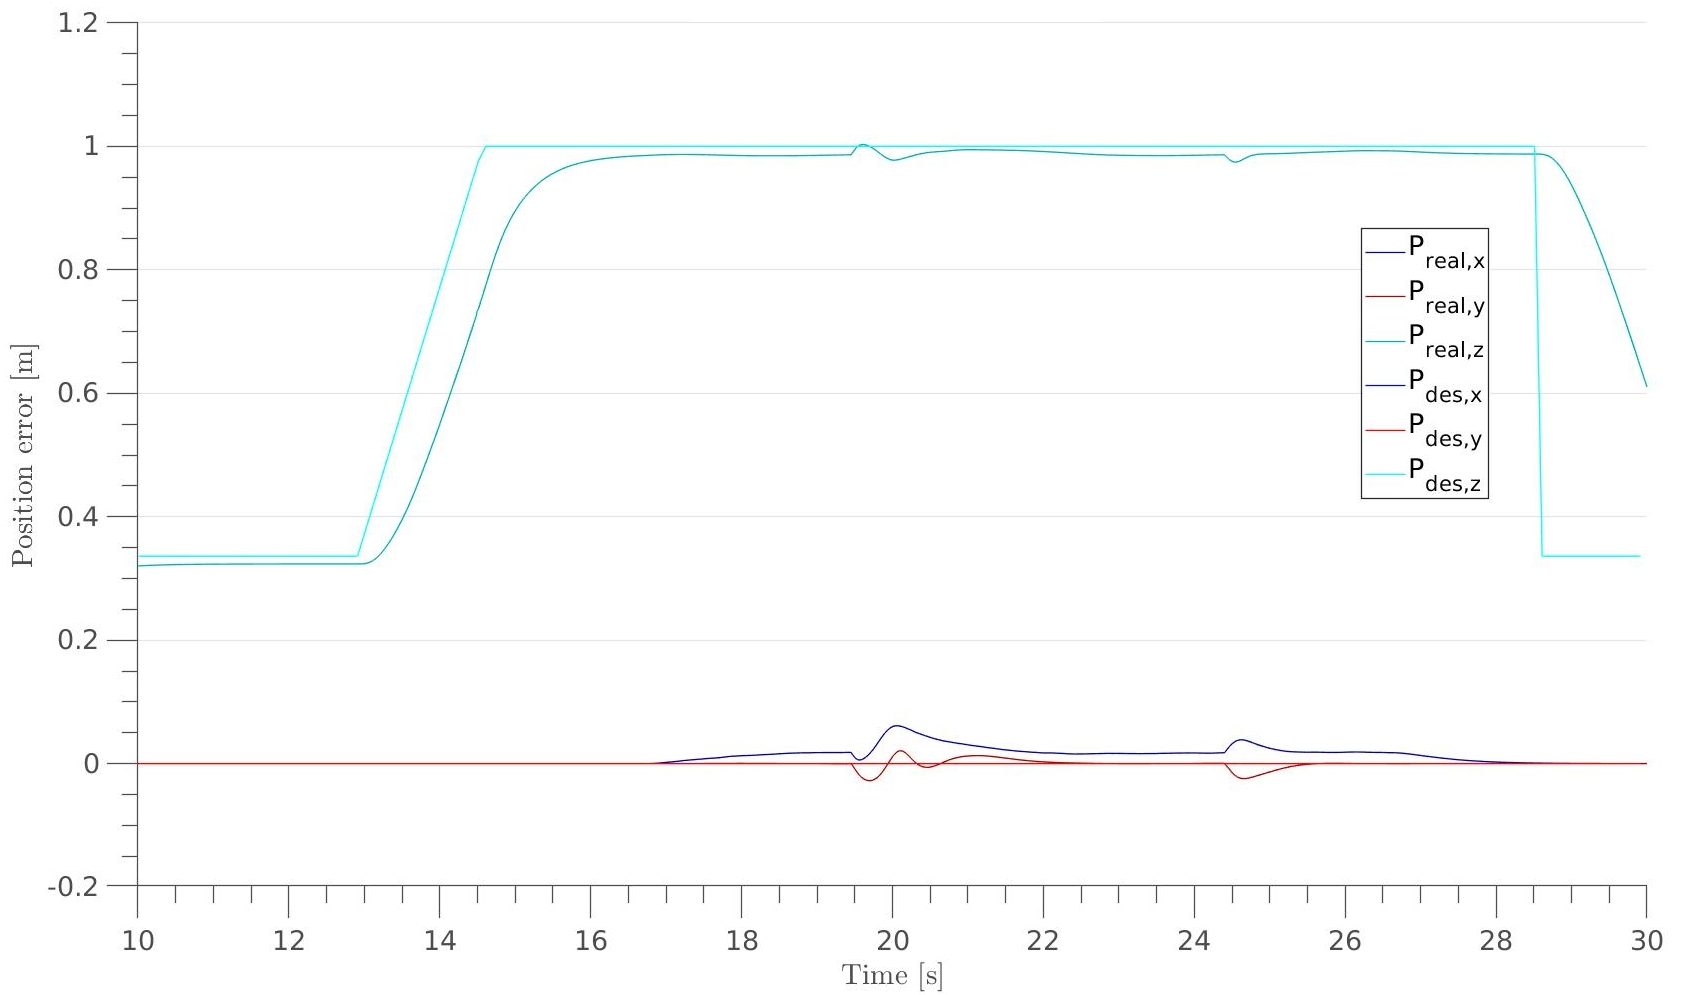
\includegraphics[width=1.0\linewidth]{images/Voliro_pitch_position.jpg}
    \caption{Trajectory tracking for Voliro performing a full pitch flip.}
    \label{fig:Voliro_position_pitch}
  \end{center}
\end{figure}

\begin{figure}[!ht]
  \begin{center}
    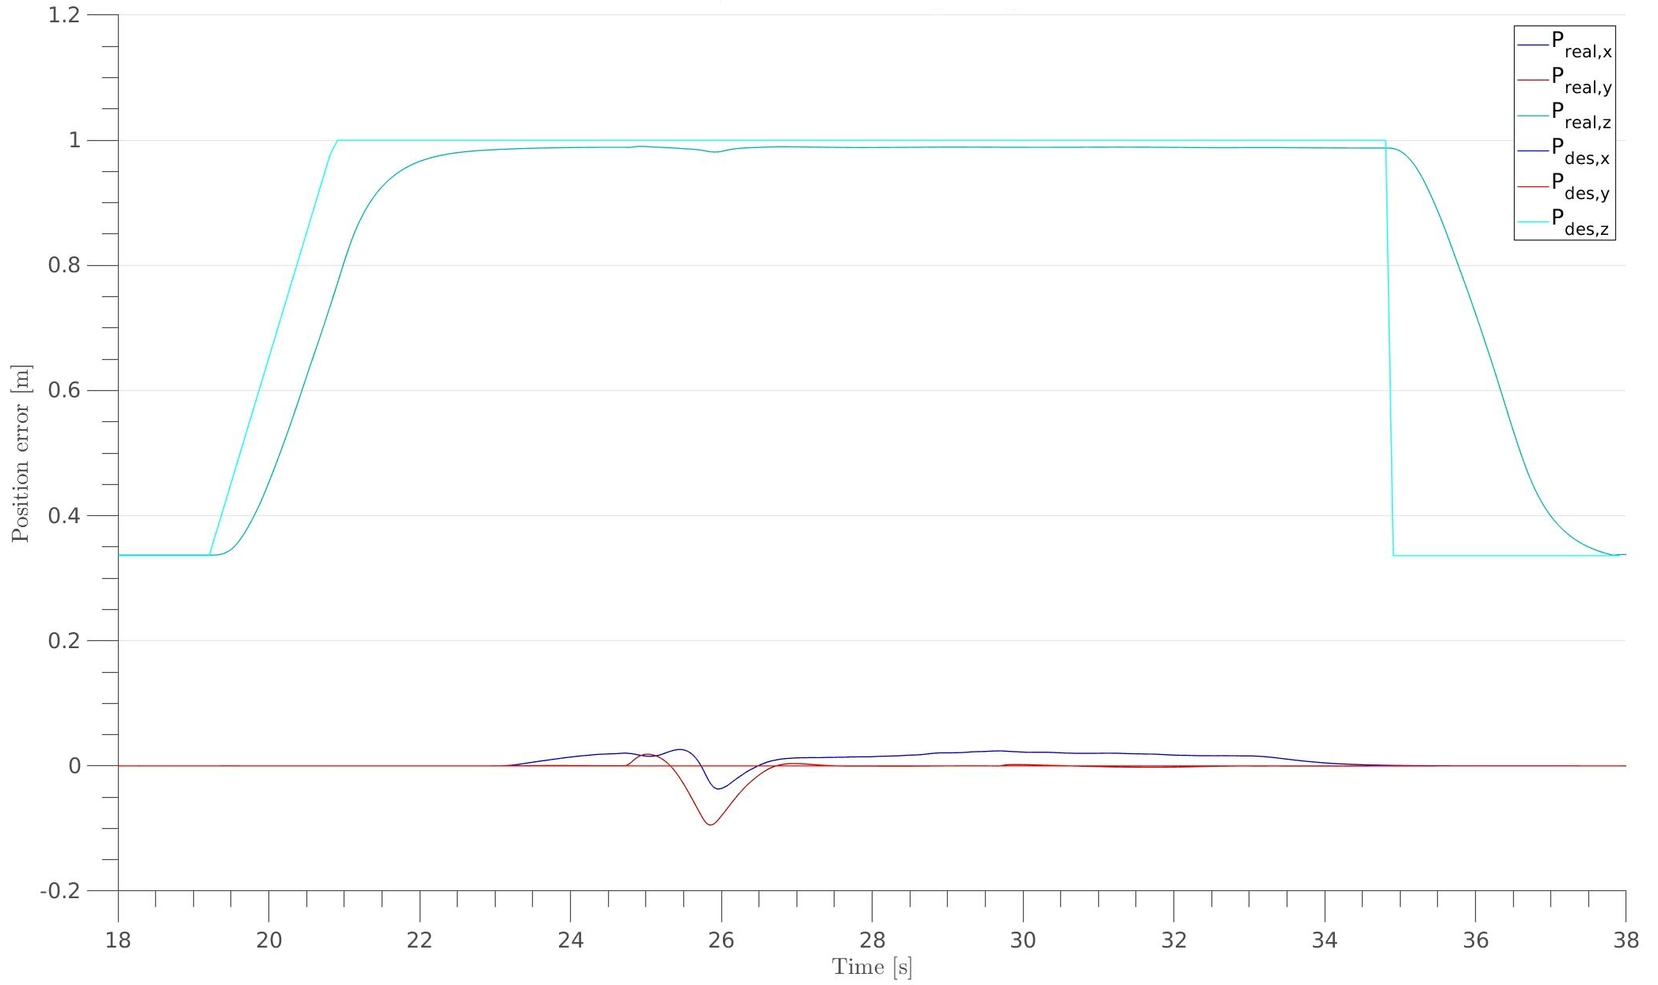
\includegraphics[width=1.0\linewidth]{images/Hexa_pitch_position.jpg}
    \caption{Trajectory tracking for the optimal hexa-copter performing a full pitch flip.}
    \label{fig:Hexa_position_pitch}
  \end{center}
\end{figure}

\begin{figure}[!ht]
  \begin{center}
    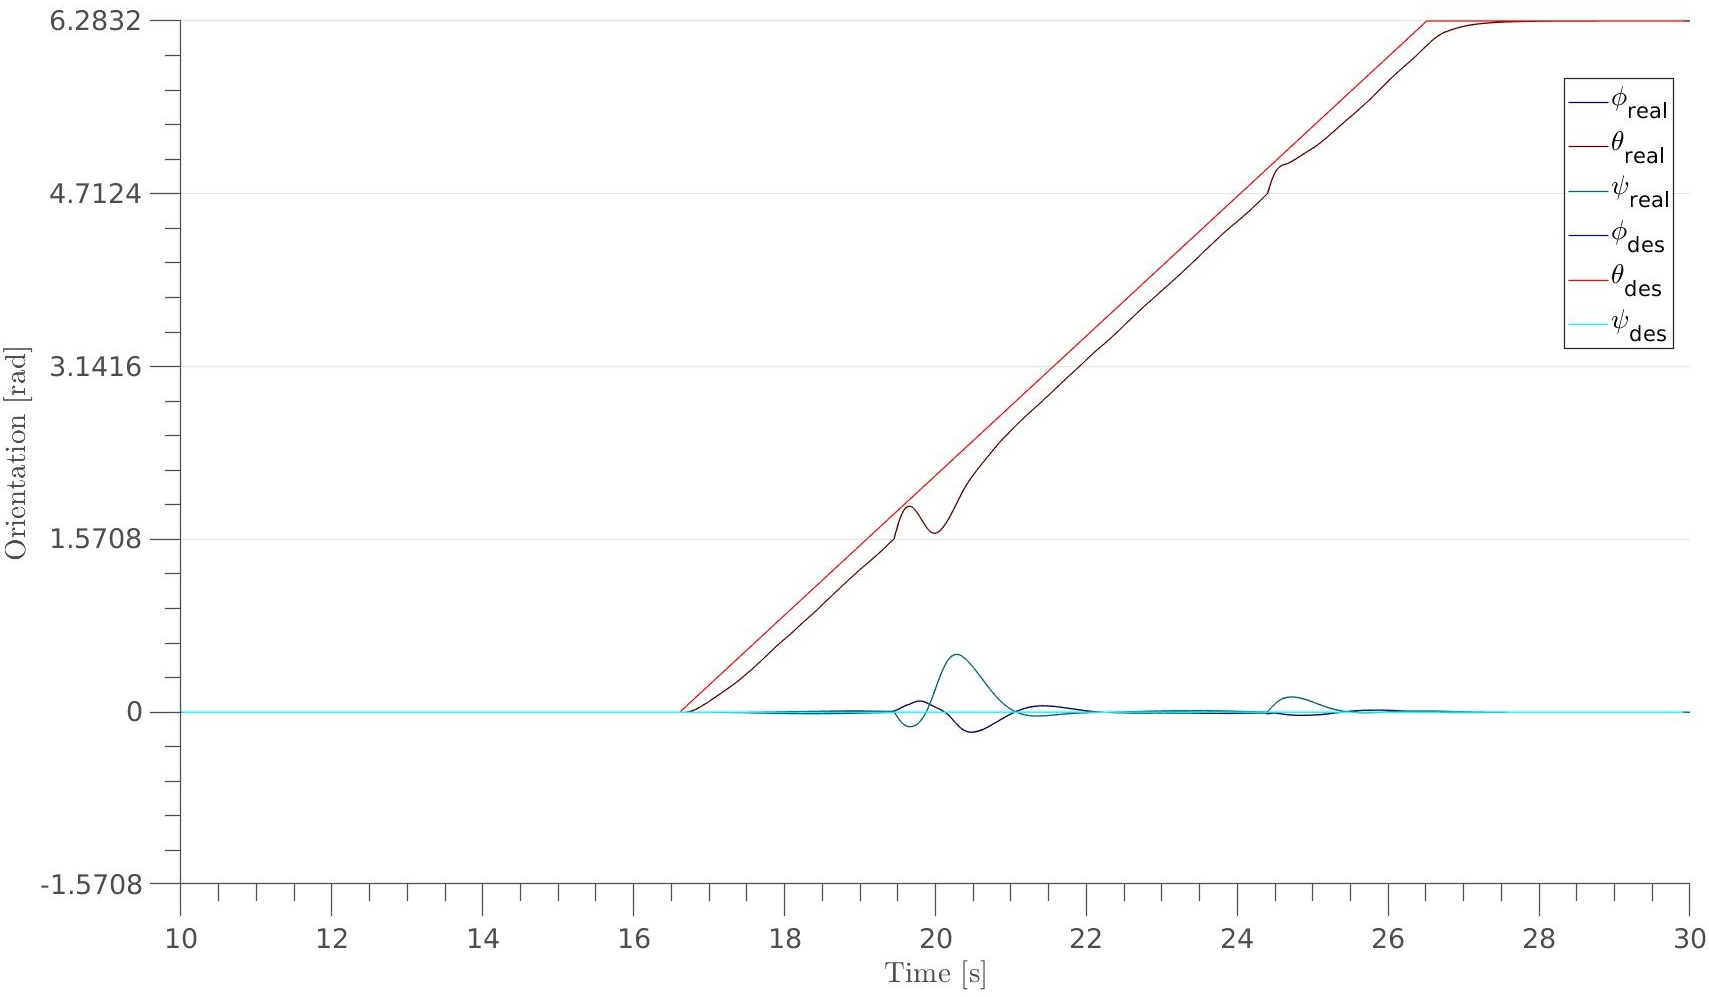
\includegraphics[width=1.0\linewidth]{images/Voliro_pitch_angle.jpg}
    \caption{Pitch, roll and yaw angle tracking for Voliro performing a full pitch flip.}
    \label{fig:Voliro_angle_pitch}
  \end{center}
\end{figure}

\begin{figure}[!ht]
  \begin{center}
    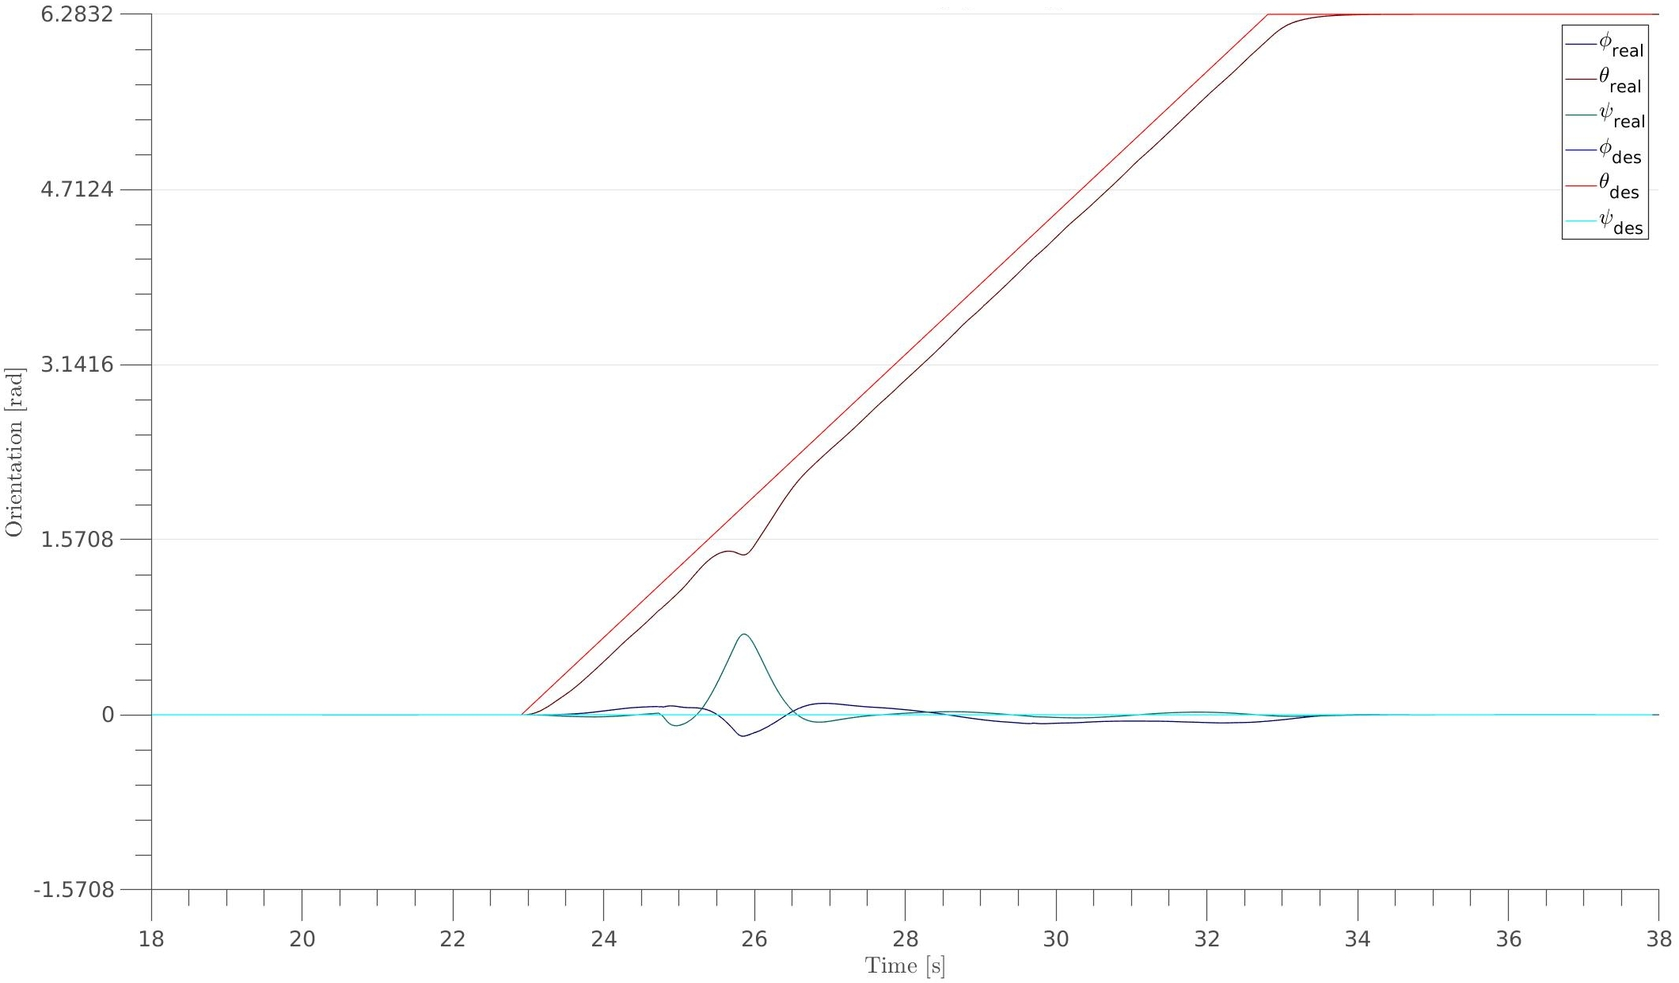
\includegraphics[width=1.0\linewidth]{images/Hexa_pitch_angle.jpg}
    \caption{Pitch, roll and yaw angle tracking for the optimal hexa-copter performing a full pitch flip.}
    \label{fig:Hexa_angle_pitch}
  \end{center}
\end{figure}

\clearpage

\section{Hepta-copter}
\label{sec:hepta_copter_sim}

\begin{figure}[!ht]
    \begin{center}
    \begin{minipage}[t]{0.495\textwidth}
      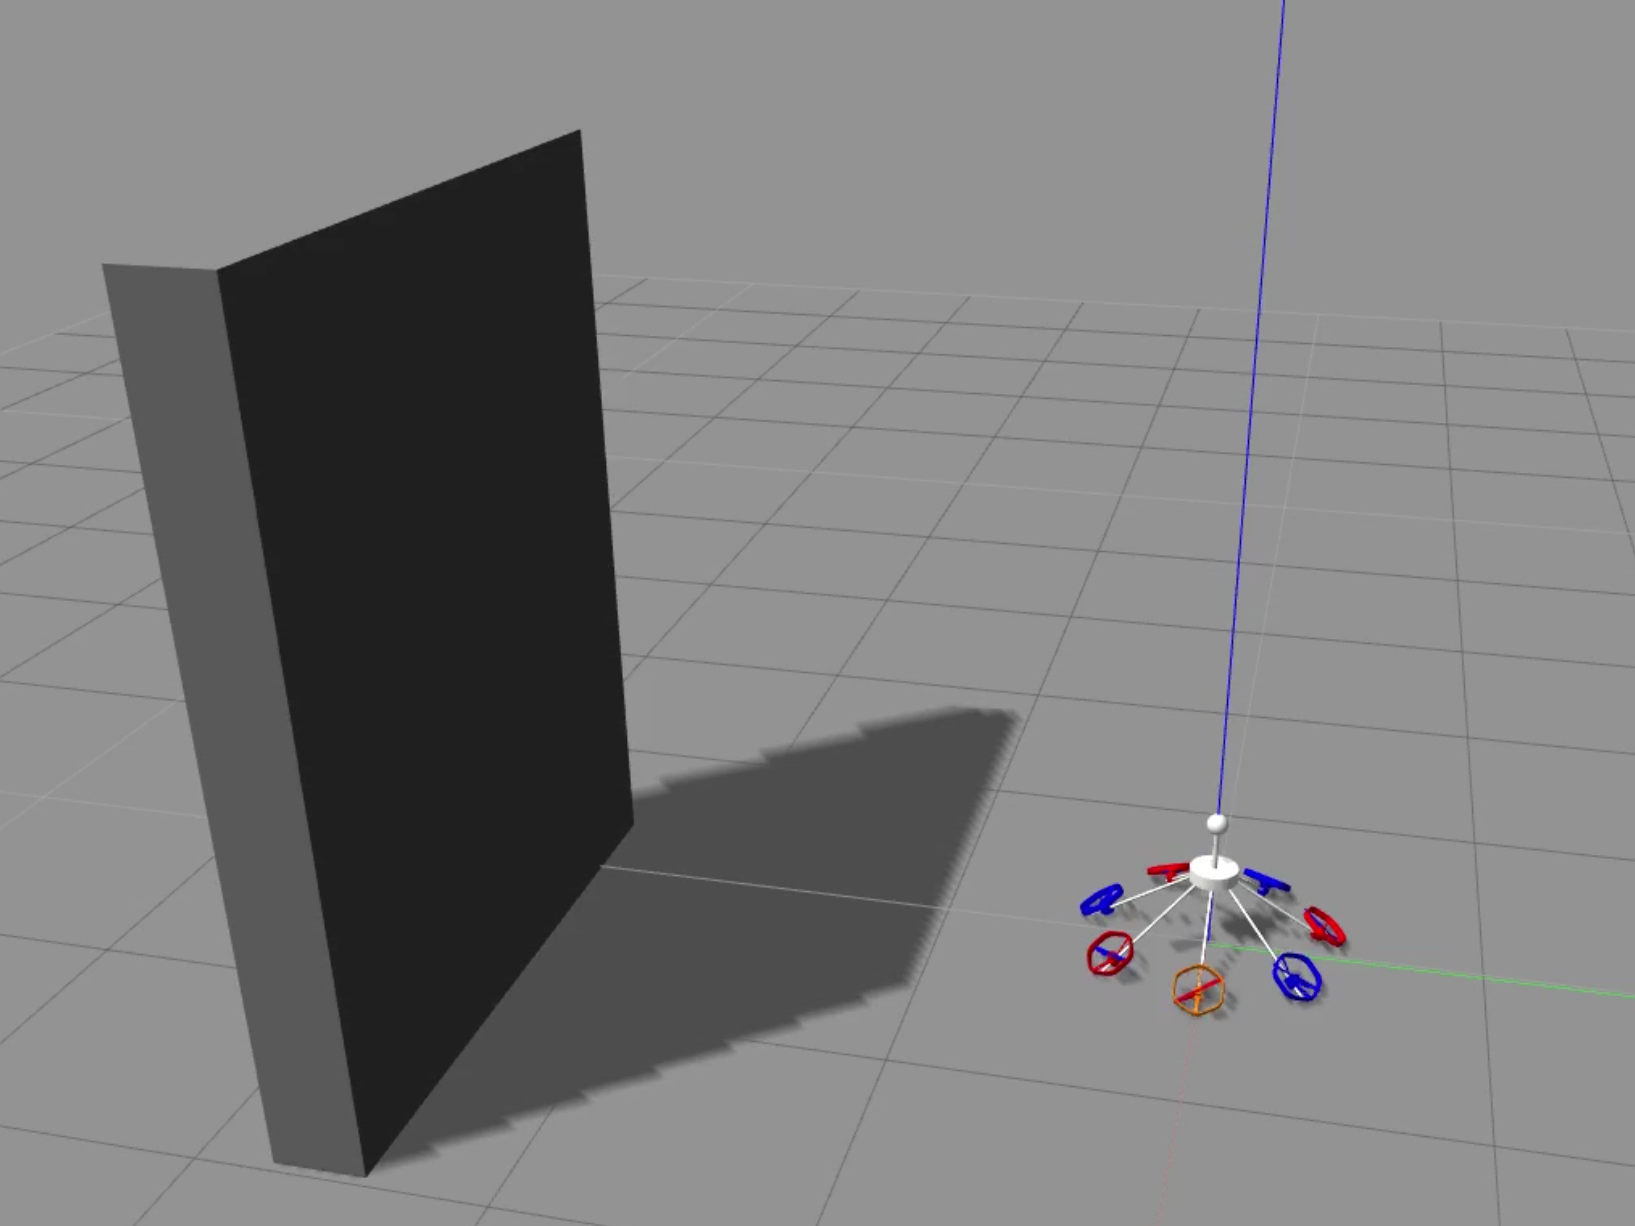
\includegraphics[width=\linewidth]{images/Selection_009.png}
    \end{minipage}
    \hfill
    \begin{minipage}[t]{0.495\textwidth}
      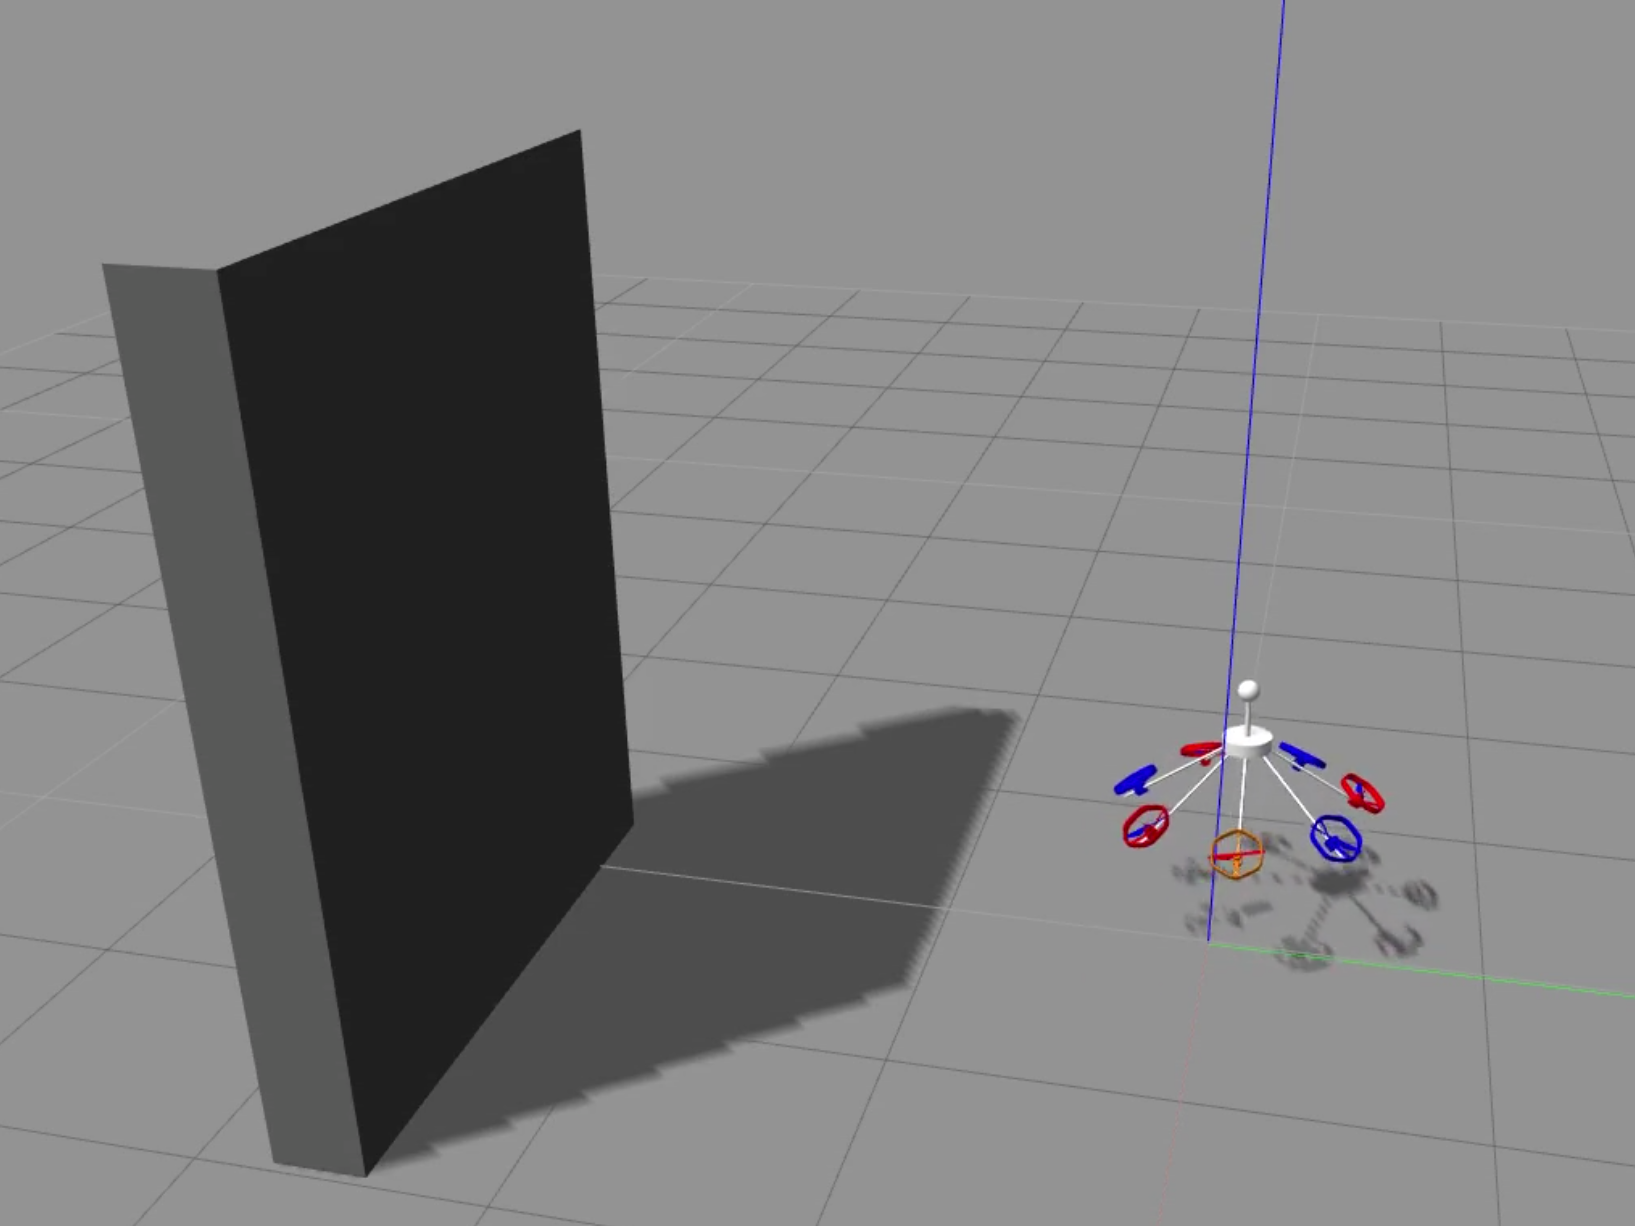
\includegraphics[width=\linewidth]{images/Selection_010.png}
    \end{minipage}
    \hfill
    \begin{minipage}[t]{0.495\textwidth}
      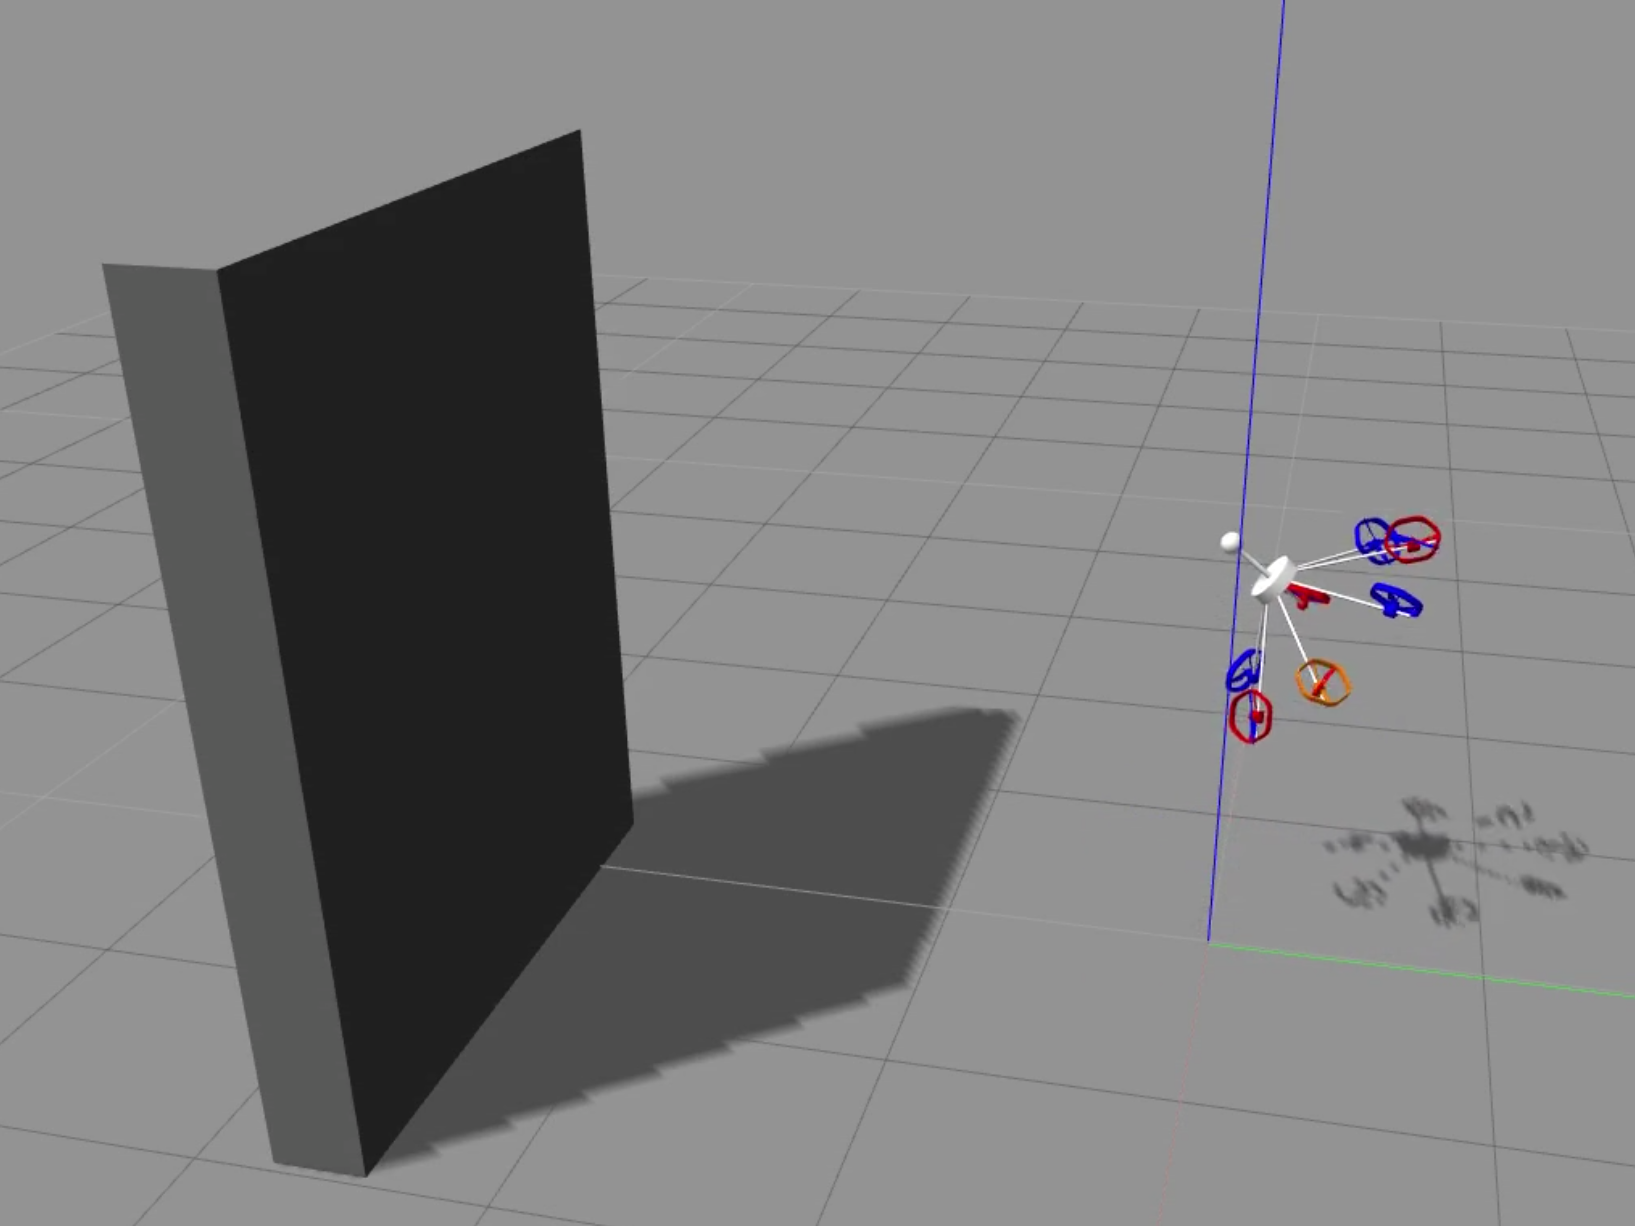
\includegraphics[width=\linewidth]{images/Selection_011.png}
    \end{minipage}
    \hfill
    \begin{minipage}[t]{0.495\textwidth}
      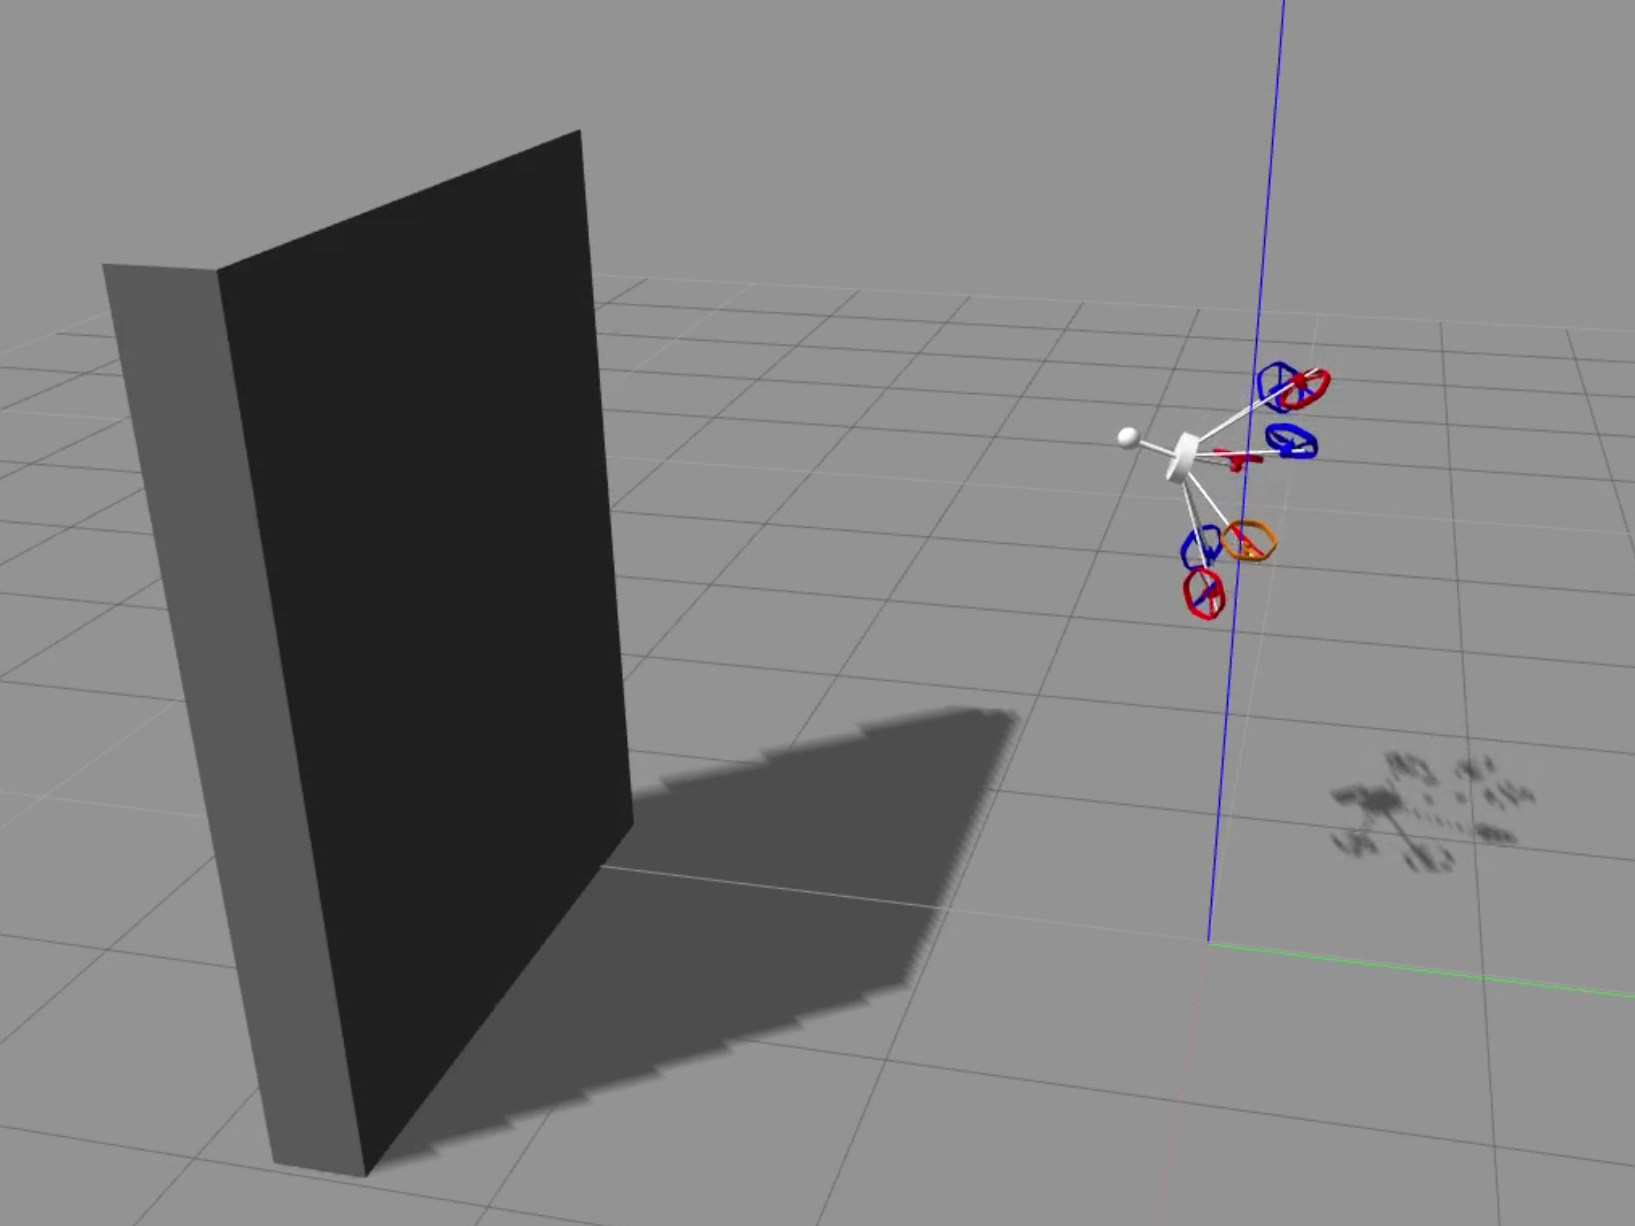
\includegraphics[width=\linewidth]{images/Selection_013.png}
    \end{minipage}
    \hfill
    \begin{minipage}[t]{0.495\textwidth}
      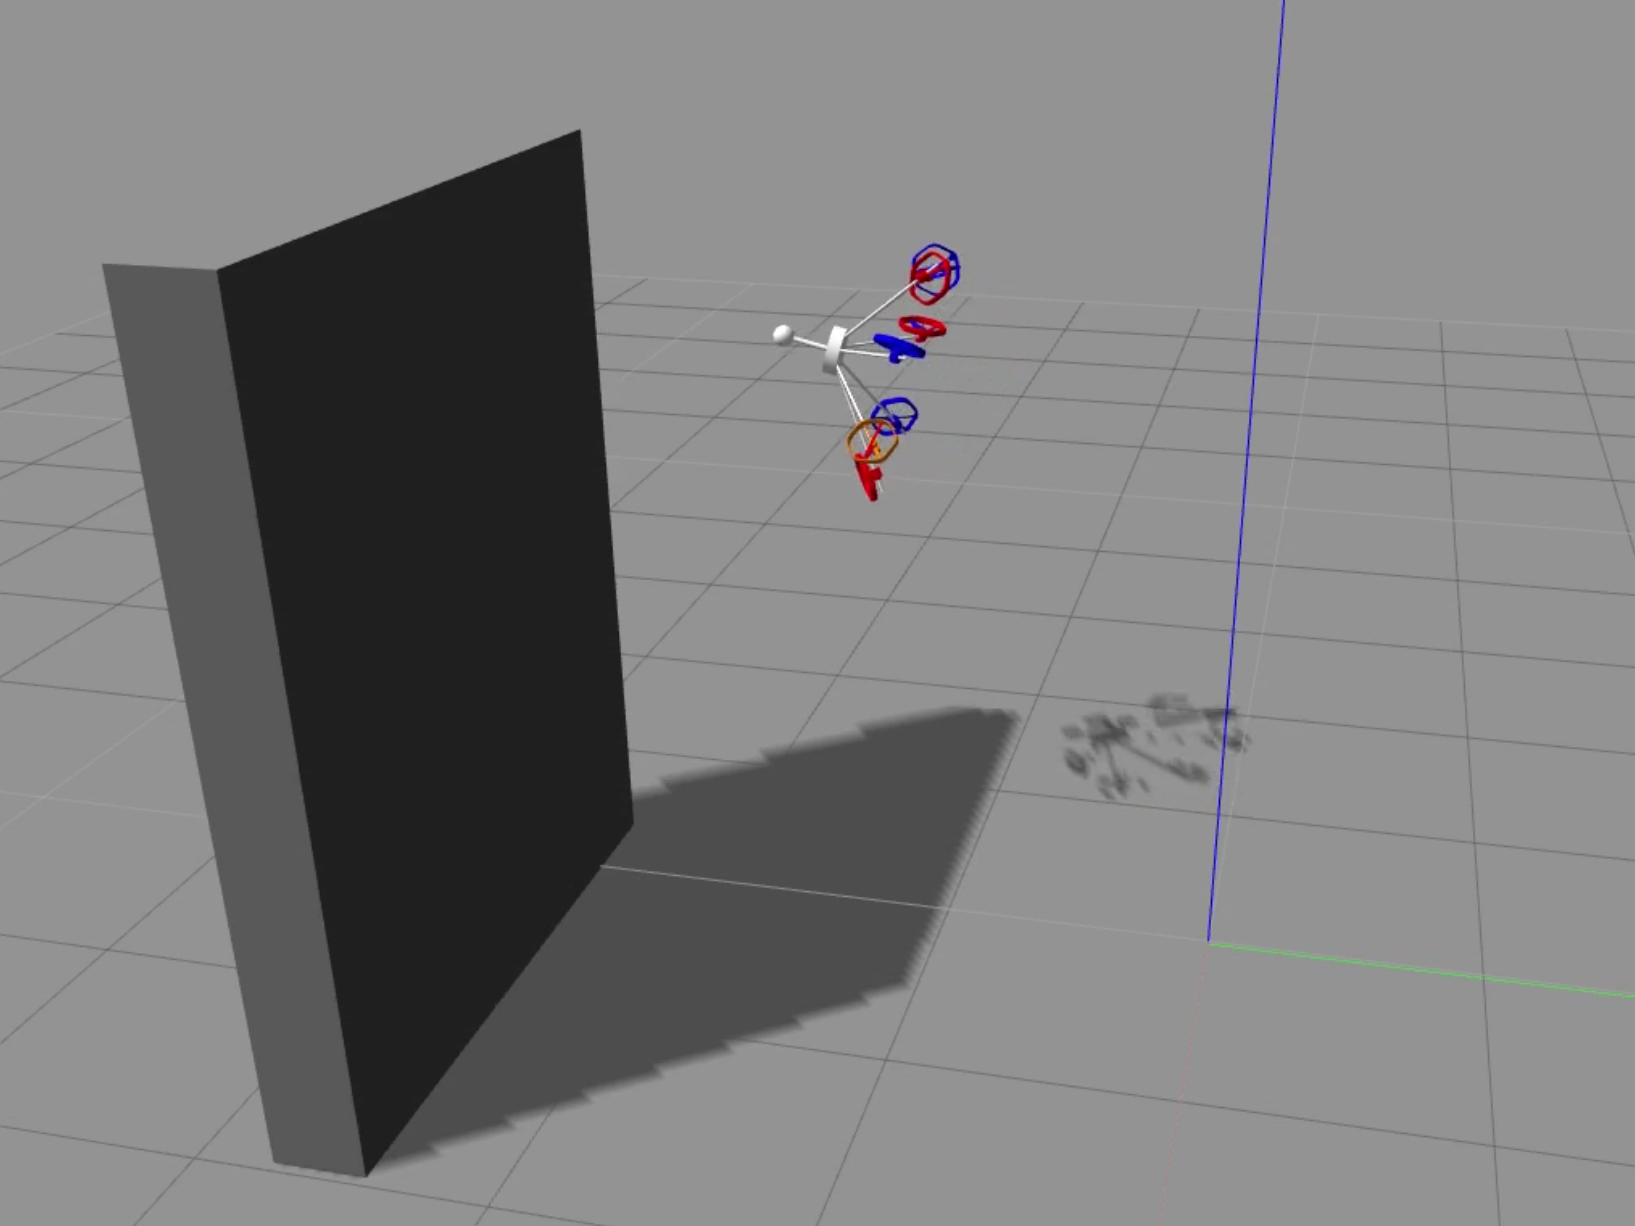
\includegraphics[width=\linewidth]{images/Selection_017.png}
    \end{minipage}
    \hfill
    \begin{minipage}[t]{0.495\textwidth}
      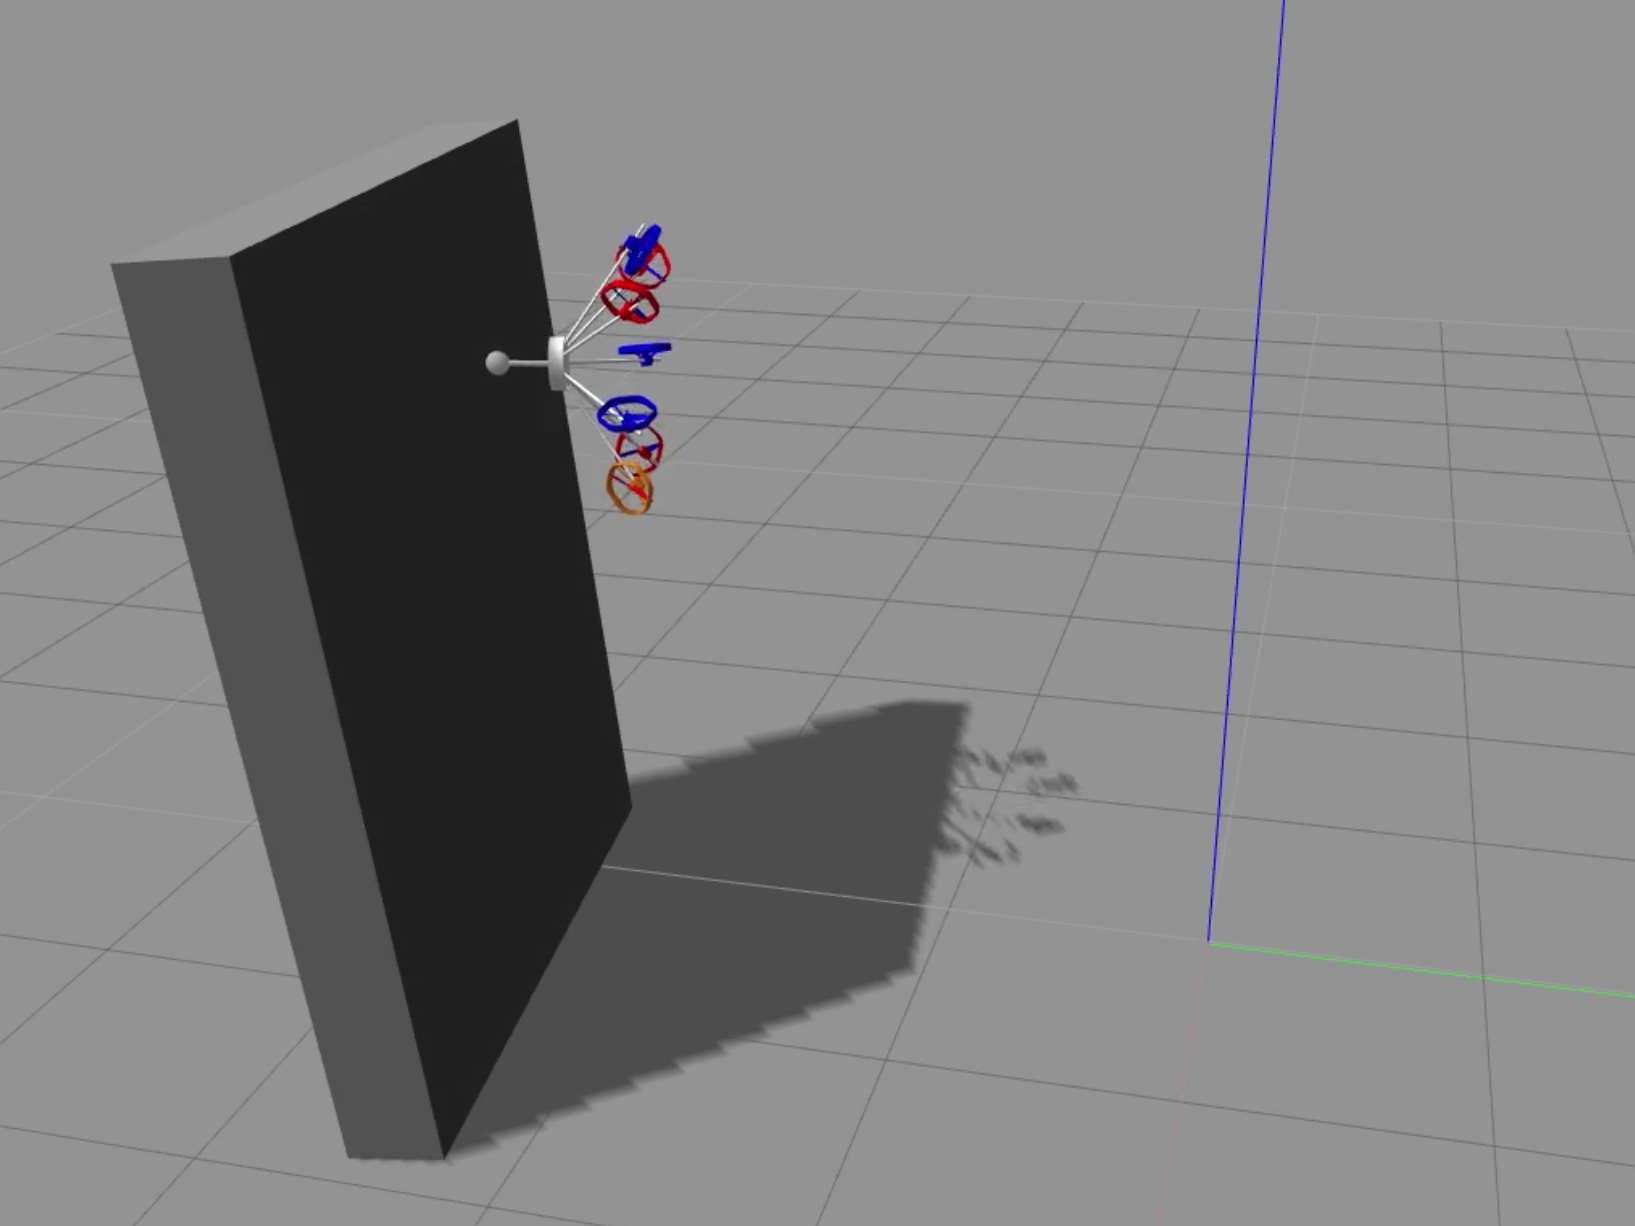
\includegraphics[width=\linewidth]{images/Selection_019.png}
    \end{minipage}
    \hfill
    \begin{minipage}[t]{0.495\textwidth}
      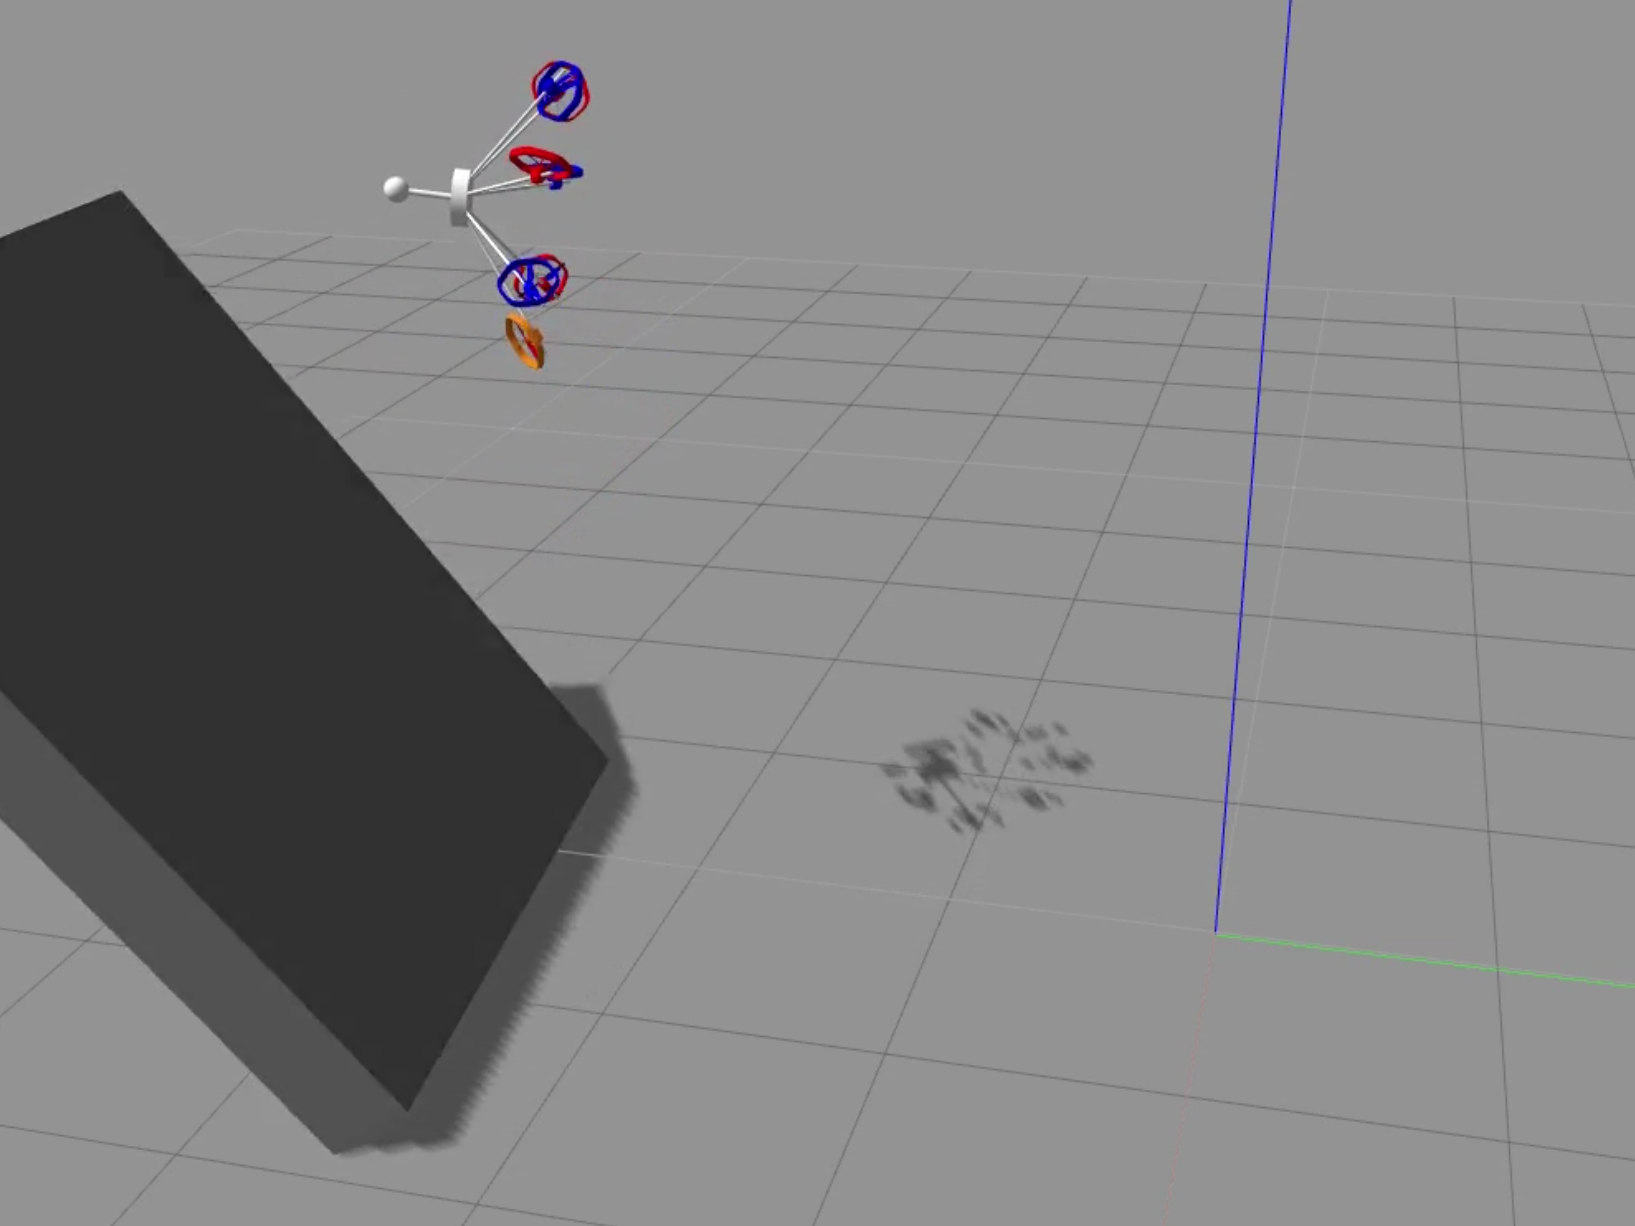
\includegraphics[width=\linewidth]{images/Selection_024.png}
    \end{minipage}
    \hfill
    \begin{minipage}[t]{0.495\textwidth}
      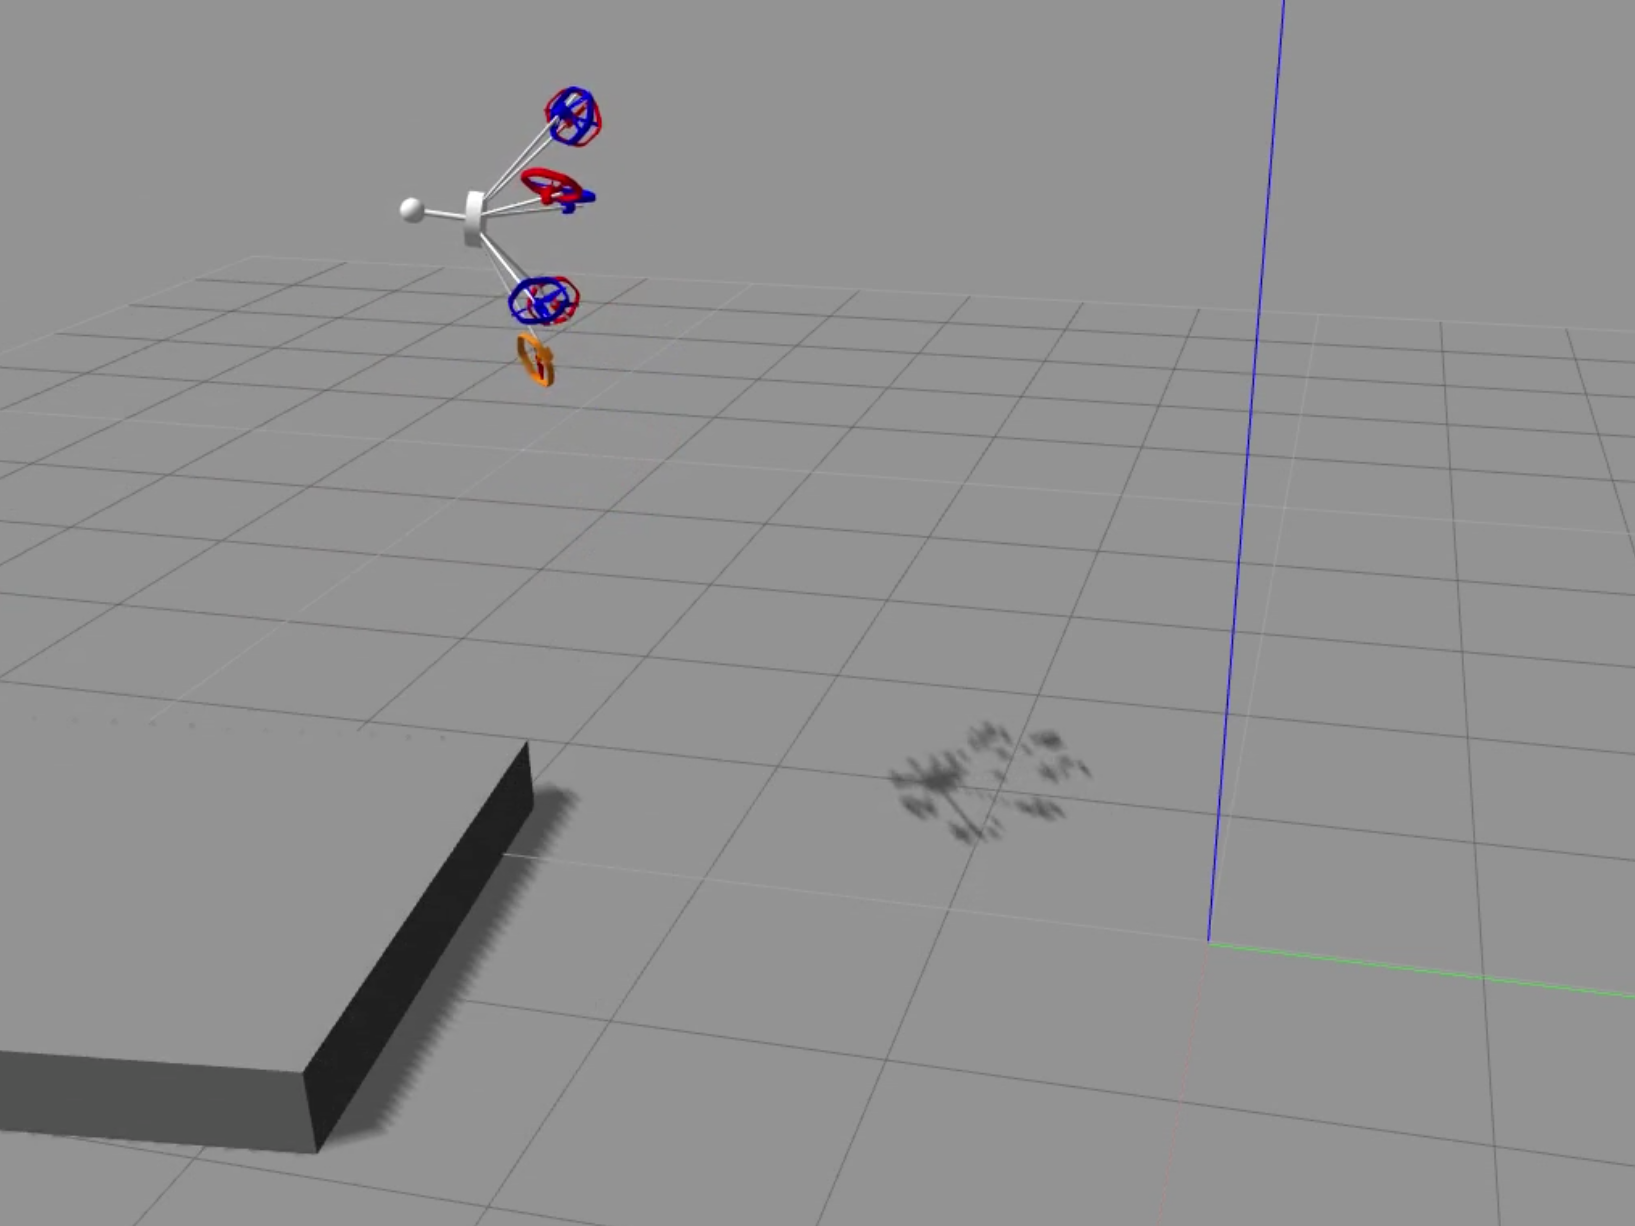
\includegraphics[width=\linewidth]{images/Selection_026.png}
    \end{minipage}
    \caption{Slideshow of an interacion between the optimal hepta-copter and a wall.}
    \label{fig:hepta_sim}
  \end{center}
\end{figure}

The slide show above illustrate a manipulation task performed with the optimal
hepta-copter design obtained in \Cref{sec:hepta_copter}. The MAV is used to
demolish a wall (see \Cref{fig:hepta_sim}) . Although it is a very light wall of
$1\ [kg]$, which falls easily on the ground this test represents quite well the
omni-directionality and the manipulation capabilities of the hepta-copter.
